
\chapter{Large sample inference}
\label{largeSampleInference}

Chapter~\ref{foundationsForInference} introduced a framework of statistical inference focused on estimation of the population mean $\mu$. Chapter~\ref{largeSampleInference} explores statistical inference for six slightly more interesting cases: differences of two population means (\ref{pairedData}, \ref{differenceOfTwoMeans}); a single population proportion (\ref{singleProportion}); differences of two population proportions (\ref{differenceOfTwoProportions}); and introduce inference tools for categorical variables with many levels (\ref{oneWayChiSquare}, \ref{twoWayTablesAndChiSquare}). For each application included in Sections~\ref{pairedData}-\ref{differenceOfTwoProportions}, we verify conditions that ensure the sampling distribution of the point estimates are nearly normal and then apply the general framework from Section~\ref{aFrameworkForInference}. Sections~\ref{oneWayChiSquare} and~\ref{twoWayTablesAndChiSquare} introduce a new distribution called the chi-square distribution, which is useful for evaluating independence among categorical variables. In Chapter~\ref{smallSampleInference} we will extend our reach to smaller samples.

%%%%%%%%%
\section{Paired data}
\label{pairedData}

Are textbooks actually cheaper online? Here we compare the price of textbooks at UCLA's bookstore and prices at Amazon.com. Seventy-three UCLA courses were randomly sampled in Spring 2010, representing less than 10\% of all UCLA courses\footnote{When a class had multiple books, only the most expensive text was considered.}. A portion of this \data{textbooks} data set is shown in Table~\ref{textbooksDF}. \vspace{2.5mm}

\begin{table}[h]
\centering
\begin{tabular}{rllrrr}
  \hline
 & deptAbbr & course & uclaNew & amazNew & diff \\ 
  \hline
1 & Am Ind &  C170 & 27.67 & 27.95 & -0.28 \\ 
  2 & Anthro & 9 & 40.59 & 31.14 & 9.45 \\ 
$\vdots$ & $\vdots$ & $\vdots$ & $\vdots$ & $\vdots$ & $\vdots$ \\
%  72 & Wom Std & M144 & 23.76 & 18.72 & 5.04 \\ 
  73 & Wom Std & 285 & 27.70 & 18.22 & 9.48 \\ 
   \hline
\end{tabular}
\caption{Three cases of the \data{textbooks} data set.}
\label{textbooksDF}
\end{table}\vspace{-2.5mm}

\subsection{Paired observations and samples}

Each textbook has two corresponding prices in the data set: one for the UCLA bookstore and one for Amazon. Therefore, each textbook price from the UCLA bookstore has a natural correspondence with a textbook price from Amazon. When two sets of observations have this special correspondence, they are said to be \term{paired}.

\begin{termBox}{\tBoxTitle{Paired data}
Two sets of observations are \emph{paired} if each observation in one set has a special correspondence or connection with exactly one observation in the other data set.}
\end{termBox}

To analyze paired data, it is often useful to look at the difference in outcomes of each pair of observations. In the \data{textbook} data set, we look at the difference in prices, which is represented as the \var{diff} variable in the \data{textbooks} data. Here the differences are taken as
\begin{eqnarray*}
\text{UCLA price} - \text{Amazon price}
\end{eqnarray*}
for each book. It is important that we always subtract using a consistent order; here Amazon prices are always subtracted from UCLA prices. A histogram of these differences is shown in Figure~\ref{diffInTextbookPricesS10}. Using differences between paired observations is a common and useful way to analyze paired data.
\begin{figure}
\centering
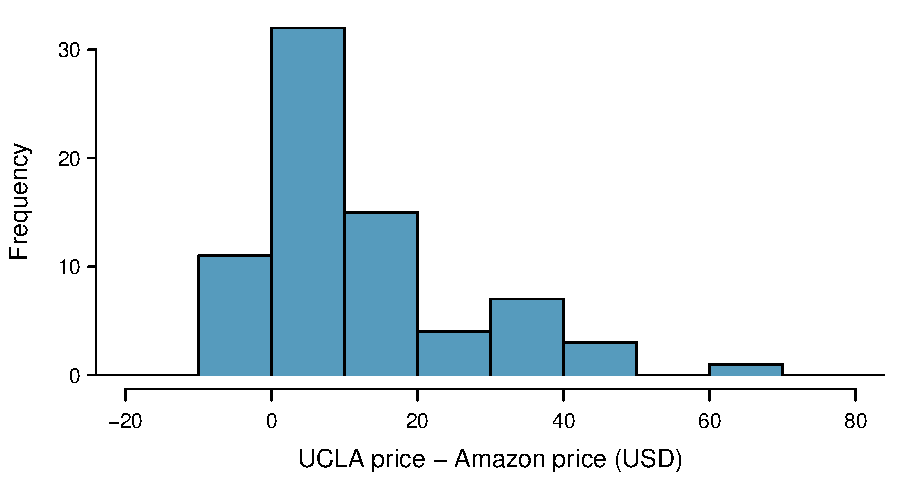
\includegraphics[width=0.8\textwidth]{05/figures/textbooksS10/diffInTextbookPricesS10}
\caption{Histogram of the difference in price for each book sampled.}
\label{diffInTextbookPricesS10}
\end{figure}

\begin{exercise}
The first difference shown in Table~\ref{textbooksDF} is computed as $27.67-27.95=-0.28$. Verify the other two differences in the table are computed correctly.
\end{exercise}

\subsection{Inference for paired data}

To analyze a paired data set, we use the exact same tools we developed in Chapter~4 and we simply apply them to the differences in the paired observations.
\begin{table}[hh]
\centering
\begin{tabular}{ccccc}
\hline
$n_{_{diff}}$	&\hspace{3mm}& $\bar{x}_{_{diff}}$	&\hspace{3mm}& $s_{_{diff}}$ \vspace{1mm}\\
73			&& 12.76				&& 14.26 \\
\hline
\end{tabular}
\caption{Summary statistics for the \var{diff} variable. There were 73 books, so there are 73 differences.}
\label{textbooksSummaryStats}
\end{table}

\begin{example}{Set up and implement a hypothesis test to determine whether, on average, there is a difference between Amazon's price for a book and the UCLA bookstore's price.}
\label{htForDiffInUCLAAndAmazonTextbookPrices}
There are two scenarios: there is no difference or there is a difference in average prices. The \emph{no difference} scenario is always the null hypothesis:
\begin{itemize}
\item[$H_0$:] $\mu_{diff}=0$. There is no difference in the average textbook price. The notation $\mu_{diff}$ is used as a notational reminder that we should only work with the difference in prices.
\item[$H_A$:] $\mu_{diff} \neq 0$. There is a difference in average prices.
\end{itemize}
Can the normal model be used to describe the sampling distribution of $\bar{x}_{diff}$? We must check that the \var{diff} data meet the conditions established in Chapter~\ref{foundationsForInference}. The observations are based on a simple random sample from less than 10\% of all books sold at the bookstore, so independence is reasonable. There is skew in the differences (Figure~\ref{diffInTextbookPricesS10}), however, it is not extreme. There are also more than 50 differences. Thus, we can conclude the sampling distribution of $\bar{x}_{diff}$ is nearly normal.

We compute the standard error associated with $\bar{x}_{diff}$ using the standard deviation of the differences and the number of differences:
$$SE_{\bar{x}_{diff}} = \frac{s_{diff}}{\sqrt{n_{diff}}} = \frac{14.26}{\sqrt{73}} = 1.67$$
To visualize the p-value, the sampling distribution of $\bar{x}_{diff}$ is drawn under the condition as though $H_0$ was true, which is shown in Figure~\ref{textbooksS10HTTails}. The p-value is represented by the two (very) small tails.
\begin{figure}
\centering
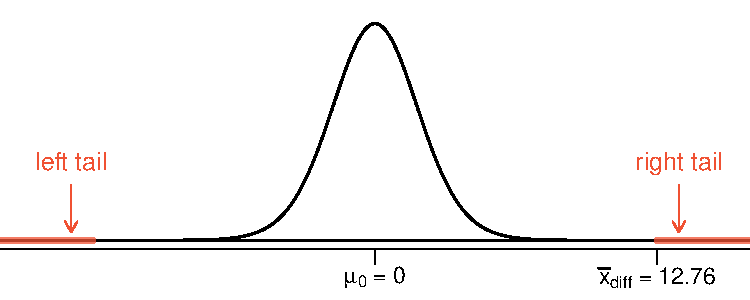
\includegraphics[width=0.65\textwidth]{05/figures/textbooksS10/textbooksS10HTTails}
\caption{Sampling distribution for the mean difference in book prices, if the true average difference is zero.}
\label{textbooksS10HTTails}
\end{figure}

To find the tail areas, we compute the test statistic, which is the Z score of $\bar{x}_{diff}$ under the condition $\mu_{diff} = 0$:
$$Z = \frac{\bar{x}_{diff} - 0}{SE_{x_{diff}}} = \frac{12.76 - 0}{1.67} = 7.59$$
This Z score is so large it isn't even in the table, which ensures the single tail area will be 0.0002 or smaller. Since the p-value is both tails and the normal distribution is symmetric, the p-value can be estimated as twice the one-tail area:
$$\text{p-value} = 2*(\text{one tail area}) \approx 2*0.0002 = 0.0004$$
Because the p-value is less than 0.05, we reject the null hypothesis. We have found convincing evidence that Amazon is, on average, cheaper than the UCLA bookstore for UCLA course textbooks.
\end{example}

\begin{exercise}
Create a 95\% confidence interval for the average price difference between books at the UCLA bookstore and books on Amazon. Answer in the footnote\footnote{Conditions have already verified and the standard error computed in Example~\exam{htForDiffInUCLAAndAmazonTextbookPrices}. To find the interval, identify $z^{\star}$ (1.96 for 95\% confidence) and plug it, the point estimate, and the standard error into the general confidence interval formula:
$$\text{point estimate} \pm z^{\star}SE \quad\to\quad 12.76 \pm (1.96)(1.67) \quad\to\quad (9.49, 16.03)$$
We are 95\% confident that Amazon is, on average, between \$9.49 and \$16.03 cheaper than the UCLA bookstore for UCLA course books.}.
\end{exercise}

%%%%%%%%%
\section{Difference of two means}
\label{differenceOfTwoMeans}

In this section we consider a difference in two population means, $\mu_1 - \mu_2$, under the condition that the data are not paired. The methods are similar in theory but different in the details. Just as with a single sample, we identify conditions to ensure a point estimate of the difference, $\bar{x}_1 - \bar{x}_2$, is nearly normal. Next we introduce a formula for the standard error, which allows us to apply our general tools from Section~4.5.

We apply these methods to two examples: participants in the 2009 Cherry Blossom Run and newborn infants. This section is motivated by questions like ``Is there convincing evidence that newborns from mothers who smoke have a different average birth weight than newborns from mothers who don't smoke?''

\subsection{Point estimates and standard errors for differences of means}

We would like to estimate the average difference in run times for men and women using a random sample of 100 men and 80 women from the \data{run10} population. Table~\ref{cherryBlossomRun2009SampleOf180SummaryStats} presents relevant summary statistics, and box plots of each sample are shown in Figure~\ref{cbrRunTimesMenWomen}.
\begin{table}[h]
\centering
\begin{tabular}{l rr}
\hline
	&	men	&	women \\
\hline
$\bar{x}$	& 88.08	& 96.28 \\
$s$	&	15.74	& 13.66 \\
$n$	&	100		& 80    \\
\hline
\end{tabular}
\caption{Summary statistics for the run time of 180 participants in the 2009 Cherry Blossom Run.}
\label{cherryBlossomRun2009SampleOf180SummaryStats}
\end{table}
\begin{figure}
\centering
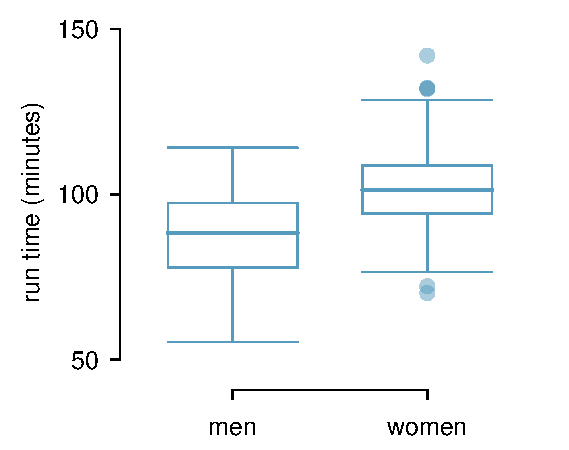
\includegraphics[width=0.5\textwidth]{05/figures/cbrRunTimesMenWomen/cbrRunTimesMenWomen}
\caption{Side-by-side box plots for the sample of 2009 Cherry Blossom Run participants.}
\label{cbrRunTimesMenWomen}
\end{figure}

The two samples are independent of one-another, so the data are not paired. Instead a point estimate of the difference in average 10 mile times for men and women, $\mu_w - \mu_m$, can be found using the two sample means:
\begin{eqnarray*}
\bar{x}_{w} - \bar{x}_{m} = 8.20
\end{eqnarray*}
Because we are examining two simple random samples from less than 10\% of the population, each sample contains at least 50 observations, and neither distribution is strongly skewed, we can safely conclude the sampling distribution of each sample means is nearly normal. Finally, because each sample is independent of the other (e.g. the data are not paired), we can conclude that the difference in sample means can be modeled using a normal distribution\footnote{Probability theory guarantees that the difference of two independent normal random variables is also normal. Because each sample mean is nearly normal and observations in the samples are independent, we are assured the difference is also nearly normal.}.

\begin{termBox}{\tBoxTitle{Conditions for normality of $\bar{x}_1 - \bar{x}_2$}
If the sample means, $\bar{x}_1$ and $\bar{x}_2$, each meet the criteria for having nearly normal sampling distributions and the observations in the two samples are independent, then the difference in sample means, $\bar{x}_1 - \bar{x}_2$, will have a sampling distribution that is nearly normal.}
\end{termBox}

We can quantify the variability in the point estimate, $\bar{x}_{w} - \bar{x}_{m}$, using the following formula for its standard error:
\begin{eqnarray*}
SE_{\bar{x}_{w} - \bar{x}_{m}} = \sqrt{\frac{\sigma_{w}^2}{n_{w}} + \frac{\sigma_{m}^2}{n_{m}}}
\end{eqnarray*}
We usually estimate this standard error using standard deviation estimates  based on the samples:
\begin{align*}
SE_{\bar{x}_{w} - \bar{x}_{m}}
	&= \sqrt{\frac{\sigma_{w}^2}{n_{w}} + \frac{\sigma_{m}^2}{n_{m}}} \\
	&\approx \sqrt{\frac{s_{w}^2}{n_{w}} + \frac{s_{m}^2}{n_{m}}}
	= \sqrt{\frac{13.7^2}{80} + \frac{15.7^2}{100}} = 2.19
\end{align*}
Because each sample has at least 50 observations ($n_{w} = 80$ and $n_{m} = 100$), this substitution using the sample standard deviation tends to be very good.

\begin{termBox}{\tBoxTitle{Distribution of a difference of sample means}
The sample difference of two means, $\bar{x}_1 - \bar{x}_2$, is nearly normal with mean $\mu_{1}-\mu_{2}$ and estimated standard error
\begin{eqnarray}
\textstyle
SE_{\bar{x}_{1} - \bar{x}_{2}} = \sqrt{\frac{s_1^2}{n_1} + \frac{s_2^2}{n_2}}
\label{seOfDifferenceInMeans}
\end{eqnarray}
when each sample mean is nearly normal and all observations are independent.}
\end{termBox}

\subsection{Confidence interval for the difference}

When the conditions are met for the sampling distribution of $\bar{x}_{1} - \bar{x}_{2}$ to be nearly normal, we can construct a 95\% confidence interval for the difference in two means from the framework built in Chapter~\ref{foundationsForInference}. Here a point estimate, $\bar{x}_{w} - \bar{x}_{m} = 8.20$, is associated with a normal model with standard error $SE=2.19$. Using this information, the general confidence interval formula may be applied in an attempt to capture the true difference in means:
\begin{eqnarray*}
\text{point estimate} \pm z^{\star}SE \quad\to\quad 8.20 \pm 1.96*2.19 \quad\to\quad (3.91, 12.49)
\end{eqnarray*}
Based on the samples, we are 95\% confident that men ran, on average, between 3.91 and 12.49 minutes faster than women in the 2009 Cherry Blossom Run.

\begin{exercise}
What does 95\% confidence mean? Answer in the footnote\footnote{If we were to collected many such samples and create 95\% confidence intervals for each, then about 95\% of these intervals would contain the population difference, $\mu_w - \mu_m$.}.
\end{exercise}

\begin{exercise}
We may be interested in a different confidence level. Construct the 99\% confidence interval for the population difference in average run times based on the sample data. Hint in the footnote\footnote{The only thing that changes is $z^{\star}$: we use $z^{\star}=2.58$ for a 99\% confidence level. If the selection of $z^{\star}$ is confusing, see Section~4.2.4 for an explanation.}.
\end{exercise}

\subsection{Hypothesis tests based on a difference in means}

A data set called \data{babySmoke} represents a random sample of 150 cases of mothers and their newborns in North Carolina over a year. Four cases from this data set are represented in Table~\ref{babySmokeDF}. We are particularly interested in two variables: \var{weight} and \var{smoke}. The \var{weight} variable represents the weights of the newborns and the \var{smoke} variable describes which mothers smoked during pregnancy. We would like to know if there is convincing evidence that newborns from mothers who smoke have a different average birth weight than newborns from mothers who don't smoke? We will answer this question using a hypothesis test. The smoking group includes 50 cases and the nonsmoking group contains 100 cases, represented in Figure~\ref{babySmokePlotOfTwoGroupsToExamineSkew}.
\begin{table}[h]
\centering
\begin{tabular}{rrrrrll}
  \hline
 & fAge & mAge & weeks & weight & sexBaby & smoke \\ 
  \hline
1 & NA & 13 &  37 & 5.00 & female & nonsmoker \\ 
  2 & NA & 14 &  36 & 5.88 & female & nonsmoker \\ 
  3 & 19 & 15 &  41 & 8.13 & male & smoker \\ 
  $\vdots$ &   $\vdots$ &   $\vdots$ &   $\vdots$ &   $\vdots$ &   $\vdots$ \\
  150 & 45 & 50 &  36 & 9.25 & female & nonsmoker \\ 
   \hline
\end{tabular}
\caption{Four cases from the \data{babySmoke} data set. An observation listed as ``NA'' means that particular piece of data is missing.}
\label{babySmokeDF}
\end{table}

\begin{figure}[h]
\centering
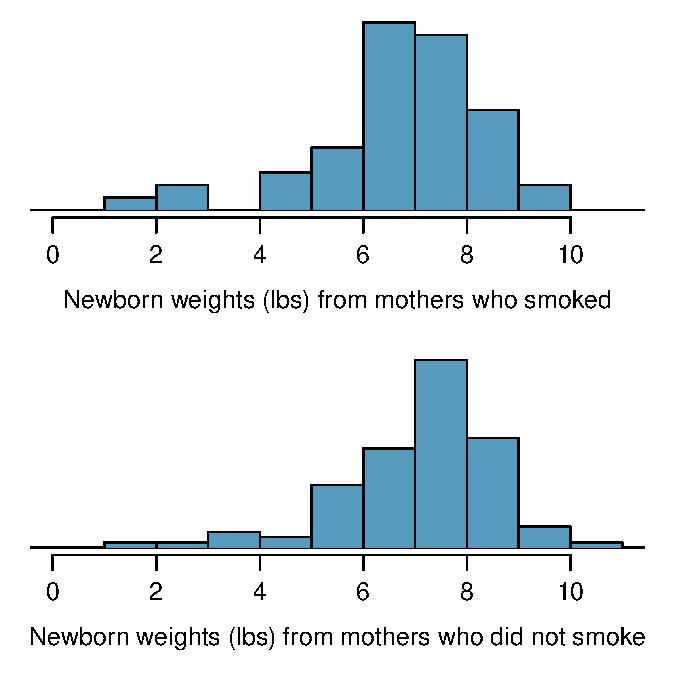
\includegraphics[width=0.6\textwidth]{05/figures/babySmokePlotOfTwoGroupsToExamineSkew/babySmokePlotOfTwoGroupsToExamineSkew}
\caption{The top panel represents birth weights for infants whose mothers smoked. The bottom panel represents the birth weights for infants whose mothers who did not smoke.}
\label{babySmokePlotOfTwoGroupsToExamineSkew}
\end{figure}

\pagebreak

\begin{example}{Set up appropriate hypotheses to evaluate whether there is a relationship between a mother smoking and average birth weight.}\label{babySmokeHTForWeight}
The null hypothesis represents the case of no difference between the groups.
\begin{itemize}
\setlength{\itemsep}{0mm}
\item[$H_0$:] There is no difference in average birth weight for newborns from mothers who did and did not smoke. In statistical notation: $\mu_{n} - \mu_{s} = 0$, where $\mu_{n}$ represents non-smoking mothers and $\mu_s$ represents mothers who smoked.
\item[$H_A$:] there is some difference in average newborn weights from mothers who did and did not smoke ($\mu_{n} - \mu_{s} \neq 0$).
\end{itemize}
\end{example}

Summary statistics are shown for each sample in Table~\ref{summaryStatsOfBirthWeightForNewbornsFromSmokingAndNonsmokingMothers}. Because each sample is simple random and consists of less than 10\% of all such cases, the observations are independent. Additionally, each sample size is at least 50 and neither sample distribution is strongly skewed (see Figure~\ref{babySmokePlotOfTwoGroupsToExamineSkew}), so both sample means are associated with a nearly normal distribution.
\begin{table}[h]
\centering
\begin{tabular}{lrr}
	& \resp{smoker} & \resp{nonsmoker} \\
\hline
mean & 6.78 & 7.18 \\
st. dev. & 1.43 & 1.60 \\
samp. size & 50 & 100 \\
\hline
\end{tabular}
\caption{Summary statistics for the \data{babySmoke} data set.}
\label{summaryStatsOfBirthWeightForNewbornsFromSmokingAndNonsmokingMothers}
\end{table}

\begin{exercise} \label{pointEstimateDistributionAndSEForBabySmokeData}
(a)~What is the point estimate of the population difference, $\mu_{n} - \mu_{s}$? (b)~Can we use a normal distribution to model this difference? (c)~Compute the standard error of the point estimate from part (a). Answers in the footnote\footnote{(a)~The difference in sample means is an appropriate point estimate: $\bar{x}_{n} - \bar{x}_{s} = 0.40$. (b)~Because the samples are independent and each sample mean is nearly normal, their difference is also nearly normal. (c)~The standard error of the estimate can be estimated using Equation~(\ref{seOfDifferenceInMeans}):
\begin{eqnarray*}
SE = \sqrt{\frac{\sigma_n^2}{n_n} + \frac{\sigma_s^2}{n_s}}
	\approx \sqrt{\frac{s_n^2}{n_n} + \frac{s_s^2}{n_s}}
	= \sqrt{\frac{1.60^2}{100} + \frac{1.43^2}{50}}
	= 0.26
\end{eqnarray*}
The sample standard deviations can be used because we have large sample sizes and neither distribution is too strongly skewed.}.
\end{exercise}

\begin{example}{If the null hypothesis was true, what would be the expected value of the point estimate from Exercise~\ref{pointEstimateDistributionAndSEForBabySmokeData}? And the standard deviation of this estimate? Draw a picture to represent the p-value.} \label{pictureOfPValueForEstimateOfDiffOfMeansOfBirthWeights}
If the null hypothesis was true, then we expect to see a difference near 0. The standard error corresponds to the standard deviation of the point estimate: 0.26. To depict the p-value, we draw the distribution of the point estimate as though $H_0$ was true and shade areas representing at least as much evidence against $H_0$ as what was observed. Both tails are shaded because it is a two-sided test.
\begin{center}
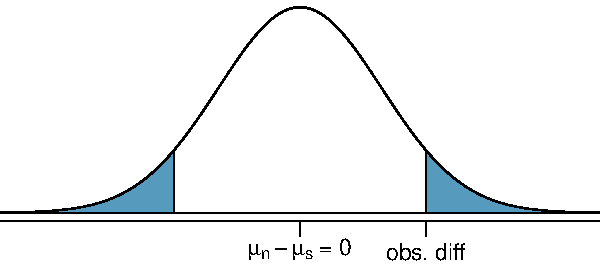
\includegraphics[width=0.6\textwidth]{05/figures/distOfDiffOfSampleMeansForBWOfBabySmokeData/distOfDiffOfSampleMeansForBWOfBabySmokeData}
\end{center}
\end{example}

\begin{example}{Compute the p-value of the hypothesis test using the figure in Example~\exam{pictureOfPValueForEstimateOfDiffOfMeansOfBirthWeights} and evaluate the hypotheses using a significance level of $\alpha=0.05$.} \label{babySmokeHTForWeightComputePValueAndEvalHT}
Since the point estimate is nearly normal, we can find the upper tail using the Z score and normal probability table:
\begin{eqnarray*}
Z = \frac{0.40 - 0}{0.26} = 1.54 \quad \to \quad \text{upper tail } = 1 - 0.938 = 0.062
\end{eqnarray*}
Because this is a two-sided test and we want the area of both tails, we double this single tail to get the p-value: 0.124. This p-value is larger than the significance value, 0.05, so we fail to reject the null hypothesis. There is insufficient evidence to say there is a difference in average birth weight of newborns from mothers who did smoke during pregnancy and newborns from mothers who did not smoke during pregnancy.
\end{example}

\begin{exercise}
Does the conclusion to Example~\exam{babySmokeHTForWeightComputePValueAndEvalHT} mean that smoking and average birth weight are unrelated? Answer in the footnote\footnote{Absolutely not. It is possible that there is some difference but we did not detect it. If this is the case, we made a Type 2 Error.}.
\end{exercise}

\begin{exercise} \label{babySmokeHTIDingHowToDetectDifferences}
If we actually did make a Type 2 Error and there is a difference, what could we have done differently in data collection to be more likely to detect such a difference? Answer in the footnote\footnote{We could have collected larger samples. If the sample size is larger, we tend to have a better shot at finding a difference if one exists.}.
\end{exercise}

\subsection{Summary for inference of the difference of two means}

When considering the difference of two means, there are two common cases: the data observed may be paired or the samples may independent. The first case was treated in Section~\ref{pairedData}, where the one-sample methods were applied to the differences from the paired observations. We examined the second and more complex scenario in this section.

When applying the normal model to the point estimate $\bar{x}_1 - \bar{x}_2$ (corresponding to unpaired data), it is important to verify conditions before applying the inference framework using the normal model. First, each sample mean must meet the conditions for normality; these conditions are described in Chapter~\ref{foundationsForInference} on page~\pageref{terBoxOfCondForXBarBeingNearlyNormalAndSEBeingAccurate}. Secondly, the samples must be collected independently (e.g. not paired data). When these conditions are satisfied, the general inference tools of Chapter~\ref{foundationsForInference} may be applied.

For example, a general confidence interval takes the following form:
\begin{eqnarray*}
\text{point estimate} \pm z^{\star} SE
\end{eqnarray*}
When estimating $\mu_1 - \mu_2$, the point estimate is the difference in sample means, the value $z^{\star}$ corresponds to the confidence level, and the standard error is computed from Equation~(\ref{seOfDifferenceInMeans}) on page~\pageref{seOfDifferenceInMeans}. While the point estimate and standard error formulas change a little, the general framework for a confidence interval stays the same. This is also true in hypothesis tests for differences of means.

In a hypothesis test, we apply the standard framework and use the specific formulas for the point estimate and standard error of a difference in two means. The test statistic represented by the Z score may be computed as
\begin{eqnarray*}
Z = \frac{\text{point estimate} - \text{null value}}{SE}
\end{eqnarray*}
When assessing the difference in two means, the point estimate takes the form $\bar{x}_1 - \bar{x}_2$, and the standard error again takes the form of Equation~(\ref{seOfDifferenceInMeans}) on page~\pageref{seOfDifferenceInMeans}. Finally, the null value is the difference in sample means under the null hypothesis. Just as in Chapter~\ref{foundationsForInference}, the test statistic $Z$ is used to identify the p-value.

\subsection{Examining the standard error formula}

The formula for the standard error of the difference in two means is similar to the formula for other standard errors. Recall that the standard error of a single mean, $\bar{x}_1$, can be approximated by
\begin{eqnarray*}
SE_{\bar{x}_1} = \frac{s_1}{\sqrt{n_1}}
\end{eqnarray*}
where $s_1$ and $n_1$ represent the sample standard deviation and sample size.

The standard error of the difference of two sample means can be constructed from the standard errors of the separate sample means:
\begin{eqnarray}
SE_{\bar{x}_{1} - \bar{x}_{2}}
	= \sqrt{SE_{\bar{x}_1}^2 + SE_{\bar{x}_2}^2}
	= \sqrt{\frac{s_1^2}{{n_1}} + \frac{s_2^2}{{n_2}}}
\label{seOfDiffOfMeansInTermsOfSEOfIndividualMeans}
\end{eqnarray}
This special relationship follows from probability theory.

\begin{exercise} Prerequisite: Section~\ref{randomVariablesSection}.
We can rewrite Equation~(\ref{seOfDiffOfMeansInTermsOfSEOfIndividualMeans}) in a different way:
\begin{eqnarray*}
SE_{\bar{x}_{1} - \bar{x}_{2}}^2 = SE_{\bar{x}_1}^2 + SE_{\bar{x}_2}^2
\end{eqnarray*}
Explain where this formula comes from using the ideas of probability theory. Hint in the footnote\footnote{The standard error squared represents the variance of the estimate. If $X$ and $Y$ are two random variables with variances $\sigma_x^2$ and $\sigma_y^2$, what is the variance of $X-Y$?}.
\end{exercise}


%%%%%%%%%
\section{Single population proportion}
\label{singleProportion}

According to a poll taken by CNN/Opinion Research Corporation in February 2010, only about 26\% of the American public trust the federal government most of the time\footnote{http://www.cnn.com/2010/POLITICS/02/23/poll.government.trust/index.html}. This poll included responses of 1,023 Americans.

We will find that the sampling distribution of sample proportions, like sample means, tends to be nearly normal when the sample size is sufficiently large.

\subsection{Identifying when a sample proportion is nearly normal}

A sample proportion can be described as a sample mean. If we represent each ``success'' as a 1 and each ``failure'' as a 0, then the sample proportion is the mean of these numerical outcomes:
\begin{eqnarray*}
\hat{p} = \frac{0 + 0 + 1 + \cdots + 0}{1023} = 0.26
\end{eqnarray*}
The distribution of $\hat{p}$ is nearly normal when the distribution of 0's and 1's is not too strongly skewed (in the case of a proportion, we mean there are almost no 0's or almost no 1's in the sample) or the sample size is sufficiently large. The most common guideline for sample size and skew when working with proportions is to ensure that we expect to observe a minimum number of successes and failures, typically at least 10 of each.

\begin{termBox}{\tBoxTitle{Conditions for the sampling distribution of $\hat{p}$ being nearly normal}
The sampling distribution for $\hat{p}$, taken from a sample of size $n$ from a population with a true proportion $p$, is nearly normal when
\begin{enumerate}
\item the sample observations are independent and
\item we expected to see at least 10 successes and 10 failures in our sample, i.e. $np\geq10$ and $n(1-p)\geq10$. This is called the \term{success-failure condition}.
\end{enumerate}
If these conditions are met, then the sampling distribution of $\hat{p}$ is nearly normal with mean $p$ and standard error
\begin{eqnarray}
SE_{\hat{p}} = \sqrt{\frac{p(1-p)}{n}}
\label{seOfPHat}
\end{eqnarray}}
\end{termBox}\marginpar[\raggedright\vspace{-53mm}

$\hat{p}$\vspace{0mm}\\\footnotesize sample\\proportion\vspace{3mm}\\\normalsize$p$\vspace{0mm}\\\footnotesize population\\proportion]{\raggedright\vspace{-53mm}

$\hat{p}$\vspace{0mm}\\\footnotesize sample\\proportion\vspace{3mm}\\\normalsize$p$\vspace{0mm}\\\footnotesize population\\proportion}

Typically we do not know the true proportion, $p$, so must substitute some value to check conditions and to estimate the standard error. For confidence intervals, usually $\hat{p}$ is used to check the success-failure condition and compute the standard error. For hypothesis tests, typically the null value -- that is, the proportion claimed in the null hypothesis -- is used in place of $p$. Examples are presented for each of these cases in Sections~\ref{confIntForPropSection} and~\ref{htForPropSection}.

\begin{tipBox}{\tipBoxTitle{Reminder on checking independence of observations}
If our data come from a simple random sample and consist of less than 10\% of the population, then the independence assumption is reasonable. Alternatively, if the data come from a random process, we must evaluate the independence condition more carefully.}
\end{tipBox}

\subsection{Confidence intervals for a proportion}
\label{confIntForPropSection}

We may want a confidence interval for the proportion of Americans who trust federal officials most of the time. Our estimate, based on a sample of size $n = 1023$ from the CNN poll, is $\hat{p} = 0.26$. To use the general confidence interval formula from Section~\ref{aFrameworkForInference}, we must check the conditions to ensure that the sampling distribution of $\hat{p}$ is nearly normal, and we must determine the standard error of the estimate.

The data are based on a simple random sample and consist of far fewer than 10\% of the U.S. population, so independence is confirmed. The sample size must also be sufficiently large, which is checked via the success-failure condition: there were approximately $1023*\hat{p}=266$ ``successes'' and $1023*(1-\hat{p})=757$ ``failures'' in the sample, both easily greater than 10.

With the conditions met, we are assured that the sampling distribution of $\hat{p}$ is nearly normal. Next, a standard error for $\hat{p}$ is needed, and then we can employ the usual method to construct a confidence interval.

\begin{exercise} \label{seOfPropOfAmericansWhoDoNotTrustFedOfficials}
Estimate the standard error of $\hat{p}=0.26$ using Equation~(\ref{seOfPHat}). Because $p$ is unknown and the standard error is for a confidence interval, use $\hat{p}$ in place of $p$.  Answer in the footnote\footnote{$SE = \sqrt{\frac{p(1-p)}{n}} \approx \sqrt{\frac{0.26(1-0.26)}{1023}} = 0.014$}.
\end{exercise}

\begin{example}{Construct a 95\% confidence interval for $p$, the proportion of Americans who trust federal officials most of the time.}
Using the standard error estimate from Exercise~\exer{seOfPropOfAmericansWhoDoNotTrustFedOfficials}, the point estimate 0.26, and $z^{\star} = 1.96$ for a 95\% confidence interval, the general confidence interval formula from Section~\ref{aFrameworkForInference} may be used:
\begin{eqnarray*}
\text{point estimate } \pm z^{\star}SE \quad\to\quad 0.26 \pm 1.96*0.014 \quad\to\quad (0.233, 0.287)
\end{eqnarray*}
We are 95\% confident that the true proportion of Americans who trusted federal officials most of the time (in February 2010) is between 0.233 and 0.287. If the proportion has not changed since this poll, not many Americans are very trusting of their federal government.
\end{example}

\begin{termBox}{\tBoxTitle[]{Constructing a confidence interval for a proportion}
\begin{itemize}
\item Verify the observations are independent and also verify the success-failure condition using $\hat{p}$.
\item If the conditions are met, the sampling distribution of $\hat{p}$ may be well-approximated by the normal model.
\item Construct the standard error using $\hat{p}$ in place of $p$ and apply the general confidence interval formula.
\end{itemize}}
\end{termBox}

\subsection{Hypothesis testing for a proportion}
\label{htForPropSection}

To apply the normal distribution framework to the context of a hypothesis test for a proportion, the independence and success-failure conditions must be satisfied. In a hypothesis test, the success-failure condition is checked using the null proportion: we verify $np_0$ and $n(1-p_0)$ are at least 10, where $p_0$ is the null value.

\begin{exercise}
Deborah Toohey is running for Congress, and her campaign manager claims she has more than 50\% support from the district's electorate. Set up a hypothesis test to evaluate this (one-sided) claim. Answer in the footnote\footnote{Is there convincing evidence that the campaign manager is correct? $H_0: p = 0.50$, $H_A: p > 0.50$.}.
\end{exercise}

\begin{example}{A newspaper collects a simple random sample of 500 likely voters in the district and finds Toohey's support at 52\%. Does this provide convincing evidence for the claim of Toohey's manager at the 5\% significance level?}
Because this is a simple random sample that includes fewer than 10\% of the population, the observations are independent. In a one-proportion hypothesis test, the success-failure condition is checked using the null proportion, $p_0=0.5$: $np_0 = n(1-p_0) = 500*0.5 = 250 > 10$. With these conditions verified, the normal model may be applied to $\hat{p}$.

Next the standard error can be computed. Again the null value is used because this is a hypothesis test for a single proportion.
$$SE = \sqrt{\frac{p_0*(1-p_0)}{n}} = \sqrt{\frac{0.5*(1-0.5)}{500}} = 0.022$$
A picture of the normal model is shown in Figure~\ref{pValueForCampaignManagerClaimOfMoreThan50PercentSupport} with the p-value represented. Based on the normal model, the test statistic can be computed as the Z score of the point estimate:
$$Z = \frac{\text{point estimate} - \text{null value}}{SE} = \frac{0.52 - 0.50}{0.022} = 0.89$$
The upper tail area, representing the p-value, is 0.186. Because the p-value is larger than 0.05, we failed to reject the null hypothesis. We did not find convincing evidence to support the campaign manager's claim.
\end{example}
\begin{figure}[hht]
\centering

%ZZQ Formatting
\vspace{-2.5mm}

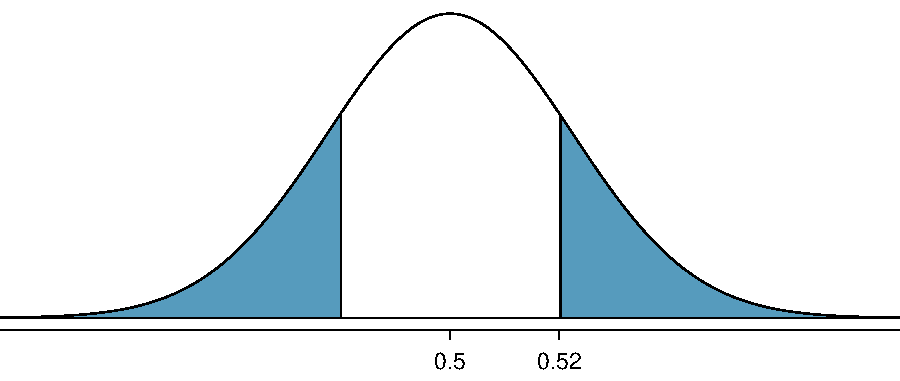
\includegraphics[width=0.4\textwidth]{05/figures/pValueForCampaignManagerClaimOfMoreThan50PercentSupport/pValueForCampaignManagerClaimOfMoreThan50PercentSupport}
\caption{Sampling distribution of the sample proportion if the null hypothesis were true. The p-value for the test is shaded.}
\label{pValueForCampaignManagerClaimOfMoreThan50PercentSupport}
\end{figure}

%ZZQ Formatting
\vspace{-3mm}

\begin{termBox}{\tBoxTitle{Hypothesis test for a proportion}
Set up hypotheses and verify the conditions using the null value, $p_0$, to ensure $\hat{p}$ is nearly normal under $H_0$. If the conditions hold, construct the standard error, again using $p_0$, and show the p-value in a drawing. Lastly, compute the p-value and evaluate the hypotheses.}
\end{termBox}

%ZZQ Formatting
\vspace{-1mm}

\subsection{Choosing a sample size when estimating a proportion}

We first encountered sample size computations in Section~\ref{sampleSizeAndPower}, which considered the case of estimating a single mean. We found that these computations were helpful in planning a study to control the uncertainty of a point estimate. The task was to find a sample size $n$ so that the sample mean would be within some margin of error $m$ of the true value with a certain level of confidence. For example, the margin of error for a point estimate using 95\% confidence is $1.96*SE$, so we had set up an equation to represent the problem:
\begin{align*}
ME = z^{\star}SE \leq m
\end{align*}
where $ME$ represented the margin of error and $z^{\star}$ was chosen to correspond to the confidence level. This problem also arises when the point estimate is a proportion instead of a mean. For instance, if we are conducting a political survey to find the proportion of folks who approve of the job the president is doing, how big of a sample do we need in order to be sure the margin of error is less than 0.04 using a 95\% confidence level?

\begin{example}{Find the smallest sample size $n$ so that the margin of error of the point estimate $\hat{p}$ will be no larger than $m=0.04$.}
This expression can be written out mathematically as follows:
\begin{align*}
ME = z^{\star}SE = 1.96*\sqrt{\frac{p(1-p)}{n}} \leq 0.04
\end{align*}
There are two unknowns: $p$ and $n$. If we have an estimate of $p$ -- perhaps from a recent poll -- we could use that value. If we have no such estimate, we must use some other value for $p$. It turns out that the margin of error is largest when $p$ is 0.5, so we typically use this \emph{worst case estimate} if no other estimate is available:
\begin{align*}
	1.96*\sqrt{\frac{0.5(1-0.5)}{n}} &\leq 0.04 \\
	1.96^2*\frac{0.5(1-0.5)}{n} &\leq 0.04^2 \\
600.25 = 1.96^2*\frac{0.5(1-0.5)}{0.04^2} &\leq n
\end{align*}
We would need at least 600.25 participants -- i.e. 601 participants -- to ensure the sample proportion is within 0.04 of the true proportion with 95\% confidence.
\end{example}

No estimate of the true proportion is required in sample size computations for a proportion, whereas an estimate of the standard deviation is always needed when computing a sample size for an error of a mean. However, if we have an estimate of the proportion, we should use it in place of the worst case estimate of the proportion, 0.5.

\begin{exercise}
A recent estimate of the President's approval rating was 47\%\footnote{Gallup Poll for President Obama's approval rating, June 13-19, 2011.}. What sample size does this estimate suggest we should use for a margin of error of 0.04 with 95\% confidence? Answer in the footnote\footnote{We complete the same computations as before, except now we use $0.47$ instead of $0.5$ for $p$:
\begin{align*}
1.96*\sqrt{\frac{p(1-p)}{n}} \approx
1.96*\sqrt{\frac{0.47(1-0.47)}{n}} &\leq 0.04 \qquad\to\qquad n \geq 598.1
\end{align*}
A sample size of 599 or more would be reasonable.}.
\end{exercise}

\begin{exercise}
A manager is about to oversee the mass production of a new tire model in her factory, and she would like to estimate what proportion of these tires will be rejected through quality control. The quality control team has monitored the last three tire models produced by the factory, failing 1.7\% of tires in the first model, 6.2\% of the second model, and 1.3\% of the third model. The manager would like to examine enough tires to estimate the failure rate of the new tire model to within about 2\% with a 90\% confidence level. Answers for parts (a) and (b) below are in the footnote\footnote{(a) We choose $z^{\star}$ to correspond to 90\% confidence instead of 95\% confidence. That is, we use 1.65 in place of 1.96. \par
(b) For the 1.7\% estimate of $p$, we estimate the appropriate sample size as follows:
\begin{align*}
1.65*\sqrt{\frac{p(1-p)}{n}} \approx
1.65*\sqrt{\frac{0.017(1-0.017)}{n}} &\leq 0.02 \qquad\to\qquad n \geq 113.7
\end{align*}
Using the estimate from the first model, we would suggest examining 114 tires (round up!). A similar computation can be accomplished using 0.062 and 0.013 for $p$: 396 and 88.}.
\begin{itemize}
\setlength{\itemsep}{0mm}
\item[(a)] This manufacturer wants to use 90\% confidence. Compared to a 95\% confidence level how will this change any sample size computations we complete?
\item[(b)] There are three different failure rates to choose from. Perform the sample size computation for each separately, and identify three sample sizes to consider.
\item[(c)] The sample sizes in (b) vary widely. Which of the three would you suggest using? What would influence your choice?
\end{itemize}
\end{exercise}

%%%%%%%%%
\section{Difference of two proportions}
\label{differenceOfTwoProportions}

We would like to make conclusions about the difference in two population proportions: $p_1 - p_2$. We consider three examples. In the first, we construct a confidence interval for the difference in support for healthcare reform between Democrats and Republicans. In the second application, a company weighs whether they should switch to a higher quality parts manufacturer. In the last example, we examine the cancer risk to dogs from the use of yard herbicides.

In our investigations, we first identify a reasonable point estimate of $p_1 - p_2$ based on the sample. You may have already guessed its form: $\hat{p}_1 - \hat{p}_2$. Next, we verify that the point estimate follows the normal model by checking conditions. Finally, we compute the estimate's standard error and apply our inferential framework, just as we have done in many cases before.

\subsection{Sampling distribution of the difference of two proportions}

We check two conditions before applying the normal model to $\hat{p}_1 - \hat{p}_2$. First, the sampling distribution for each sample proportion must be nearly normal, and secondly, the samples must be independent. Under these two conditions, the sampling distribution of $\hat{p}_1 - \hat{p}_2$ may be well approximated using the normal model.

\begin{termBox}{\tBoxTitle{Conditions for the sampling distribution of $\hat{p}_1 - \hat{p}_2$ to be normal}
The difference in two sample proportions, $\hat{p}_1 - \hat{p}_2$, tends to follow a normal model when
\begin{itemize}
\item the sampling distribution for each proportion separately follows a normal model and
\item the samples are independent.
\end{itemize}
The standard error of the difference in sample proportions is
\begin{eqnarray}
SE_{\hat{p}_1 - \hat{p}_2}
	= \sqrt{SE_{\hat{p}_1}^2 + SE_{\hat{p}_2}^2}
	= \sqrt{\frac{p_1(1-p_1)}{n_1} + \frac{p_2(1-p_2)}{n_2}}
\label{seForDiffOfProp}
\end{eqnarray}
where $p_1$ and $p_2$ represent the population proportions, and $n_1$ and $n_2$ represent the sample sizes.}
\end{termBox}

For the difference in two means, the standard error formula took the following form:
\begin{eqnarray*}
SE_{\bar{x}_{1} - \bar{x}_{2}} = \sqrt{SE_{\bar{x}_1}^2 + SE_{\bar{x}_2}^2}
\end{eqnarray*}
The standard error for the difference in two proportions takes a similar form. The reasons behind this similarity are rooted in the probability theory of Section~\ref{randomVariablesSection}.

\subsection{Intervals and tests for $p_1-p_2$}

Just as with the case of a single proportion, the sample proportions are used to verify the success-failure condition and also compute standard error when constructing confidence intervals.

\begin{example}{One way to measure how bipartisan an issue is would be to compare the issue's support by Democrats and Republicans. In a January 2010 Gallup poll, 82\% of Democrats supported a vote on healthcare in 2010 while only 20\% of Republicans support such action\footnote{\scriptsize http://www.gallup.com/poll/125030/Healthcare-Bill-Support-Ticks-Up-Public-Divided.aspx}. This support is summarized in Figure~\ref{partisanHealthCareProps}. The sample sizes were 325 and 172 for Democrats and Republicans, respectively. Create and interpret a 90\% confidence interval of the difference in support between the two parties.}
First the conditions must be verified. Because this is a random sample from less than 10\% of the population, the observations are independent, both within the samples and between the samples. The success-failure condition also holds using the sample proportions (for each sample)\footnote{Sometimes for the two proportion case, the success-failure threshold is lowered to 5. In this book, we will still use 10.}. Because our conditions are met, the normal model can be used for the point estimate of the difference in support:
$$\hat{p}_D - \hat{p}_R = 0.82 - 0.20 = 0.62$$
The standard error may be computed using Equation~(\ref{seForDiffOfProp}) with each sample proportion:
$$SE \approx \sqrt{\frac{0.82(1-0.82)}{325} + \frac{0.20(1-0.20)}{172}} = 0.037$$
For a 90\% confidence interval, we use $z^{\star} = 1.65$:
$$\text{point estimate} \pm z^{\star}SE \quad \to \quad 0.62 \pm 1.65 * 0.037 \quad \to \quad (0.56, 0.68)$$
We are 90\% confident that the difference in support for healthcare action between the two parties is between 56\% and 68\%. Healthcare is a very partisan issue, which may not be a surprise to anyone who follows the ongoing health care debates.
\end{example}

\begin{figure}
\centering
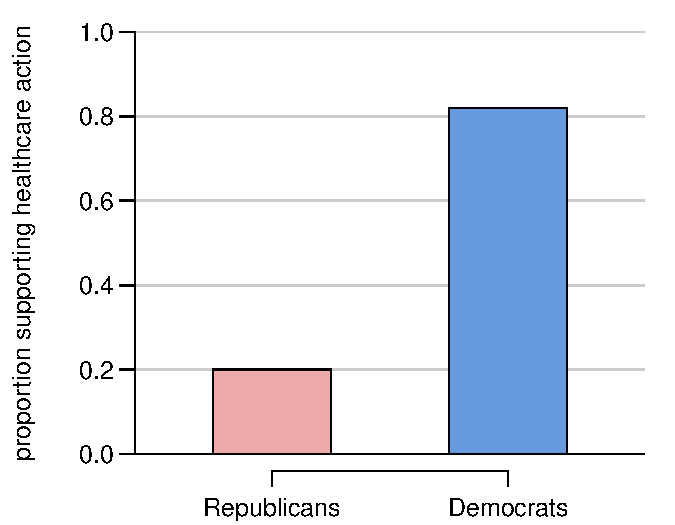
\includegraphics[width=0.45\textwidth]{05/figures/partisanHealthCareProps/partisanHealthCareProps}
\caption{Support for Congressional action on Healthcare, by political party (Gallup poll, January 2010).}
\label{partisanHealthCareProps}
\end{figure}

\pagebreak

\begin{exercise}\label{carWheelGearManufacturer}
A remote control car company is considering a new manufacturer for wheel gears. The new manufacturer would be more expensive but their higher quality gears are more reliable, resulting in happier customers and fewer warranty claims. However, management must be convinced that the more expensive gears are worth the conversion before they approve the switch. If there is strong evidence that more than a 3\% improvement in the percent of gears that pass inspection, management says they will switch suppliers, otherwise they will maintain the current supplier. Set up appropriate hypotheses for the test. Answer in the footnote\footnote{$H_0$: The higher quality gears will pass inspection no more than 3\% more frequently than the standard quality gears. $p_{highQ} - p_{standard} = 0.03$. $H_A$: The higher quality gears will pass inspection more than 3\% more often than the standard quality gears. $p_{highQ} - p_{standard} > 0.03$.}.
\end{exercise}

\begin{example}{The quality control engineer from Exercise~\exer{carWheelGearManufacturer} collects a sample of gears, examining 1000 gears from each company and finds that 899 gears pass inspection from the current supplier and 958 pass inspection from the prospective supplier. Using these data, evaluate the hypothesis setup of Exercise~\exer{carWheelGearManufacturer} using a significance level of 5\%.}
First, we check the conditions. The sample is not necessarily random, so to proceed we must assume the gears are all independent; for this sample we will suppose this assumption is reasonable, but the engineer would be more knowledgeable as to whether this assumption is appropriate. The success-failure condition also holds for each sample. Thus, the difference in sample proportions, $0.958-0.899=0.059$, can be said to come from a nearly normal distribution.

The standard error can be found using Equation~(\ref{seForDiffOfProp}):
$$SE = \sqrt{\frac{0.958(1-0.958)}{1000} + \frac{0.899(1-0.899)}{1000}} = 0.0114$$
In this hypothesis test, the sample proportions were used. We will discuss this choice more in Section~\ref{pooledHTForProportionsSection}.

Next, we compute the test statistic and use it to find the p-value, which is depicted in Figure~\ref{gearsTwoSampleHTPValueQC}.
$$Z = \frac{\text{point estimate} - \text{null value}}{SE} = \frac{0.059 - 0.03}{0.0114} = 2.54$$
Using the normal model for this test statistic, we identify the right tail area as 0.006. Since this is a one-sided test, this single tail area is also the p-value, and we reject the null hypothesis because 0.006 is less than 0.05. That is, we have statistically significant evidence that the higher quality gears actually do pass inspection more than 3\% as often as the currently used gears. Based on these results, management will approve the switch to the new supplier.
\end{example}

\begin{figure}
\centering
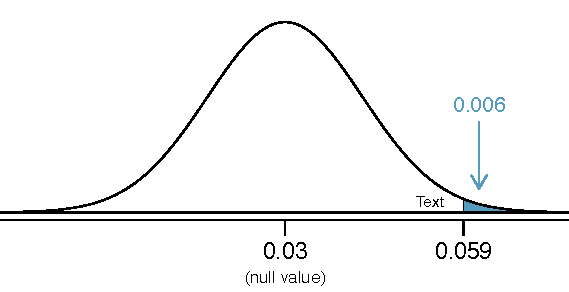
\includegraphics[width=0.5\textwidth]{05/figures/gearsTwoSampleHTPValueQC/gearsTwoSampleHTPValueQC}
\caption{Distribution of the test statistic if the null hypothesis was true. The p-value is represented by the shaded area.}
\label{gearsTwoSampleHTPValueQC}
\end{figure}

\subsection{Hypothesis testing when $H_0: p_1 = p_2$}
\label{pooledHTForProportionsSection}

Here we use a new example to examine a special estimate of standard error when $H_0: p_1 = p_2$. We investigate whether there is an increased risk of cancer in dogs that are exposed to the herbicide 2,4-dichlorophenoxyacetic acid (2,4-D). A study in 1994 examined 491 dogs that had developed cancer and 945 dogs as a control group\footnote{Hayes HM, Tarone RE, Cantor KP, Jessen CR, McCurnin DM, and Richardson RC. 1991. Case-Control Study of Canine Malignant Lymphoma: Positive Association With Dog Owner's Use of 2, 4-Dichlorophenoxyacetic Acid Herbicides. Journal of the National Cancer Institute 83(17):1226-1231.}. Of these two groups, researchers identified which dogs had been exposed to 2,4-D in their owner's yard. The results are shown in Table~\ref{24DAndCancerInDogs}.
\begin{table}[h]
\centering
\begin{tabular}{rrr}
  \hline
 & \resp{cancer} & \resp{noCancer} \\
  \hline
2,4-D & 191 & 304 \\
no 2,4-D & 300 & 641 \\
   \hline
\end{tabular}
\caption{Summary results for cancer in dogs and the use of 2,4-D by the dog's owner.}
\label{24DAndCancerInDogs}
\end{table}

\begin{exercise}
Is this study an experiment or an observational study? Answer in the footnote\footnote{The owners were not instructed to apply or not apply the herbicide, so this is an observational study. This question was especially tricky because one group was called the \emph{control group}, which is a term usually seen in experiments.}.
\end{exercise}

\begin{exercise} \label{htFor24DAndCancerInDogs}
Set up hypotheses to test whether 2,4-D and the occurrence of cancer in dogs are related. Use a one-sided test and compare across the cancer and no cancer groups. Comment and answer in the footnote\footnote{Using the proportions within the \resp{cancer} and \resp{noCancer} groups rather than examining the rates for cancer in the \resp{2,4-D} and \resp{no 2,4-D} groups may seem odd; we might prefer to condition on the use of the herbicide, which is an explanatory variable in this case. However, the cancer rates in each group do not necessarily reflect the cancer rates in reality due to the way the data were collected. For this reason, computing cancer rates may greatly alarm dog owners. \\ $H_0$: the proportion of dogs with exposure to 2,4-D is the same in the \resp{cancer} and \resp{noCancer} groups ($p_c - p_n = 0$). \\ $H_A$: the dogs with cancer are more likely to have been exposed to 2,4-D than dogs without cancer ($p_c - p_n > 0$). \\}.
\end{exercise}

\begin{example}{Are the conditions met to use the normal model and make inference on the results?}\label{condFor24DAndCancerInDogsNormalInference}
(1) It is unclear whether this is a random sample. However, if we believe the dogs in both the cancer and no cancer groups are representative of each respective population and that the dogs in the study do not interact in any way, then we may find it reasonable to assume independence between observations holds. (2) The success-failure condition holds for each sample.

Under the assumption of independence, we can use the normal model and make statements regarding the canine population based on the data.
\end{example}

In your hypotheses for Exercise~\exer{htFor24DAndCancerInDogs}, the null is that the proportion of dogs with exposure to 2,4-D is the same in each group. The point estimate of the difference in sample proportions is $\hat{p}_c - \hat{p}_n = 0.067$. To identify the p-value for this test, we first check conditions (Example~\exam{condFor24DAndCancerInDogsNormalInference}) and compute the standard error of the difference:
$$SE = \sqrt{\frac{p_c(1-p_c)}{n_c} + \frac{p_n(1-p_n)}{n_n}}$$
In a hypothesis test, the distribution of the test statistic is always examined as though the null hypothesis was true, i.e. in this case, $p_c = p_n$. The standard error formula should reflect this equality in the null hypothesis. We will use $p$ to represent the common rate of dogs that are exposed to 2,4-D in the two groups:
$$SE = \sqrt{\frac{p(1-p)}{n_c} + \frac{p(1-p)}{n_n}}$$
We don't know the exposure rate, $p$, but we can obtain a good estimate of it by \emph{pooling} the results of both samples:
$$\hat{p} = \frac{\text{\# of ``successes''}}{\text{\# of cases}} = \frac{191 + 304}{191+300+304+641} = 0.345$$
This is called the \term{pooled estimate} of the sample proportion, and we use it to compute the standard error when the null hypothesis is that $p_1 = p_2$ (e.g. $p_c = p_n$ or $p_c - p_n = 0$). We also typically use it to verify the success-failure condition.

\begin{termBox}{\tBoxTitle{Pooled estimate of a proportion}
When the null hypothesis is $p_1 = p_2$, it is useful to find the pooled estimate of the shared proportion:
\begin{eqnarray*}
\hat{p} = \frac{\text{number of ``successes''}}{\text{number of cases}} = \frac{\hat{p}_1n_1 + \hat{p}_2n_2}{n_1 + n_2}
\end{eqnarray*}
Here $\hat{p}_1n_1$ represents the number of successes in sample 1 since
\begin{eqnarray*}
\hat{p}_1 = \frac{\text{number of successes in sample 1}}{n_1}
\end{eqnarray*}
Similarly, $\hat{p}_2n_2$ represents the number of successes in sample 2.}
\end{termBox}

\begin{tipBox}{\tipBoxTitle{Using the pooled estimate of a proportion when $\mathbf{H_0: p_1 = p_2}$}
When the null hypothesis suggests the proportions are equal, we use the pooled proportion estimate ($\hat{p}$) to verify the success-failure condition and also to estimate the standard error:
\begin{eqnarray}
SE = \sqrt{\frac{\hat{p}(1-\hat{p})}{n_c} + \frac{\hat{p}(1-\hat{p})}{n_n}} 
\label{seOfDiffInPropUsingPooledEstimate}
\end{eqnarray}}
\end{tipBox}

\begin{exercise}\label{verifySEOfPooledEstimateOf24DWithCancerNoCancerDogs}
Using Equation~(\ref{seOfDiffInPropUsingPooledEstimate}), $\hat{p}=0.345$, $n_1 = 491$, and $n_2=945$, verify the estimate for the standard error is $SE = 0.026$. Next, complete the hypothesis test using a significance level of 0.05. Be certain to draw a picture, compute the p-value, and state your conclusion in both statistical language and plain language. A short answer is provided in the footnote\footnote{Compute the test statistic:
\begin{eqnarray*}
Z = \frac{\text{point estimate} - \text{null value}}{SE} = \frac{0.067 - 0}{0.026} = 2.58
\end{eqnarray*}
Looking this value up in the normal probability table: 0.9951. However this is the lower tail, and the upper tail represents the p-value: $1-0.9951 = 0.0049$. We reject the null hypothesis and conclude that dogs getting cancer and owners using 2,4-D are associated.}.
\end{exercise}



%%%%%%%%%
\section{When to retreat}

The conditions described for each statistical method ensure each test statistic follows the prescribed distribution when the null hypothesis is true. When the conditions are not met, these methods are not reliable and drawing conclusions from them is treacherous. The conditions for each test typically come in two forms.
\begin{itemize}
\setlength{\itemsep}{0mm}
\item The individual observations must be independent. A random sample from less than 10\% of the population ensures the observations are independent (not to be confused with a minimum of 10 successes and 10 failures). In experiments, other considerations must be made to ensure observations are independent. If independence fails, then advanced techniques must be used, and in some such cases, inference regarding the target population may not be possible.
\item Other conditions focus on sample size and skew. For example, if the sample size is too small or the skew too strong, then the normal model for the sample mean will fail and the methods described in this chapter are not reliable.
\end{itemize}
For analyzing smaller samples, we refer to Chapter~\ref{smallSampleInference}.% In fact, the methods of Chapter~\ref{smallSampleInference} may also be applied to large samples. However, this does not discount the utility of large sample methods, which tend to require less effort to implement.

Verification of conditions for statistical tools is always necessary. Whenever conditions are not satisfied for a statistical technique, there are three options. The first is to learn new methods that are appropriate for the data. The second route is to consult a statistician\footnote{If you work at a university, then there may be campus consulting services to assist you. Alternatively, there are many private consulting firms that are also available for hire.}. The third route is to ignore the failure of conditions. This last option effectively invalidates any analysis and may discredit novel and interesting findings.

Finally, we caution that there may be no inference tools helpful when considering data that include unknown biases, such as convenience samples. For this reason, there are books, courses, and researchers devoted to the techniques of sample and experimental design. See Sections~\ref{overviewOfDataCollectionPrinciples}-\ref{experimentsSection} for basic principles of sampling and data collection.



%%%%%%%%%
\section{Testing for goodness of fit using chi-square (special topic)}
%\section[One-way tables and the chi-square distribution (special topic)]{One-way tables and the chi-square distribution\\(special topic)}
\label{oneWayChiSquare}

In this section, we develop a method for assessing a null model when the data are binned.
This technique is commonly used in two circumstances:
\begin{itemize}
\setlength{\itemsep}{0mm}
\item Given a sample of cases that can be classified into several groups, we would like to determine if the sample is representative of the general population.
\item Evaluate whether data resemble a particular distribution, such as the normal distribution or a geometric distribution.
\end{itemize}
Each of these scenarios can be addressed using the same statistical test: a chi-square test.

In the first case, we consider data from a random sample of 275 jurors in a small county. Jurors identified their racial group, as shown in Table~\ref{juryRepresentationAndCityRepresentationForRace}, and we would like to determine if these jurors are racially representative of the population.  If the jury is representative of the population, then the proportions in the sample should roughly reflect the population of eligible jurors, i.e. registered voters.
\begin{table}[h]
\centering
\begin{tabular}{ll ccc c ll}
\hline
Race	 & \hspace{2mm} & White & Black & Hispanic & Other & \hspace{2mm} & Total \\
\hline
Representation in juries &	& 205 & 26 & 25 & 19 & & 275 \\
Registered voters	 & 		& 0.72 & 0.07 & 0.12 & 0.09 & & 1.00 \\
\hline
\end{tabular}
\vspace{-1.5mm}
\caption{Representation by race in a city's juries and population.}
\label{juryRepresentationAndCityRepresentationForRace}
\end{table}

While the proportions in the juries do not precisely represent the population proportions, it is unclear whether these data provide convincing evidence that the sample is not representative. If the jurors really were randomly sampled from the registered voters, we might expect small differences due to chance. However, unusually large differences may provide convincing evidence that the juries were not representative.

A second application, assessing the fit of a distribution, is presented at the end of this section. Daily stock returns from the S\&P500 for 1990-2009 are used to assess whether stock activity each day is independent of the stock's behavior on previous days.

In these problems, the strategy is not to assess or compare only one or two bins at a time. We would like to examine all bins simultaneously, which will require us to develop a new test statistic. While the details of the test will be new, the general ideas of hypothesis testing will be familiar.

\subsection{Creating a test statistic for one-way tables}

\begin{example}{Of the folks in the city, 275 served on a jury. If the individuals are randomly selected to serve on a jury, about how many of the 275 people would we expect to be white? How many would we expect to be black?}
About 72\% of the population is white, so we would expect about 72\% of the jurors to be white: $0.72*275 = 198$.

Similarly, we would expect about 7\% of the jurors to be black, which would correspond to about $0.07*275 = 19.25$ black jurors.
\end{example}

\begin{exercise}
Twelve percent of the population is Hispanic and 9\% represent other races. How many of the 275 jurors would we expect to be Hispanic or from another race? Answers can be found in Table~\ref{expectedJuryRepresentationIfNoBias}.
\end{exercise}

\begin{table}[h]
\centering
\begin{tabular}{ll ccc c ll}
\hline
Race	 & \hspace{2mm} & White & Black & Hispanic & Other & \hspace{2mm} & Total \\
\hline
Observed data			&	& 205 & 26	& 25 & 19	&	& 275 \\
Expected counts	 &	& 198 & 19.25 & 33 & 24.75 & & 275 \\
\hline
\end{tabular}
\vspace{-1.5mm}
\caption{Actual and expected make-up of the jurors.}
\label{expectedJuryRepresentationIfNoBias}
\end{table}

The sample proportion represented from each race among the 275 jurors was not a precise match for any ethnic group. While some sampling variation is expected, we would expect the sample proportions to be fairly similar to the population proportions if there is no bias on juries. We need to test whether the differences are strong enough to provide convincing evidence that the jurors are not a random sample. These ideas can be organized into hypotheses:
\begin{itemize}
\setlength{\itemsep}{0mm}
\item[$H_0$:] The jurors are a random sample. That is, there is no racial bias in who serves on a jury, and the observed counts reflect natural sampling fluctuation.
\item[$H_A$:] The jurors are not randomly sampled, i.e. there is racial bias in juror selection.
\end{itemize}
To evaluate these hypotheses, we quantify how different the observed counts are from the expected counts. Strong evidence for the alternative hypothesis would come in the form of unusually large deviations in the groups from what would be expected based on sampling variation alone.

\subsection{The chi-square test statistic}
\label{chiSquareTestStatistic}

In previous hypothesis tests, we constructed a test statistic of the following form:
$$ \frac{\text{point estimate} - \text{null value}}{\text{SE of point estimate}} $$
This construction was based on (1) identifying the difference between a point estimate and an expected value if the null hypothesis was true, and (2) standardizing that difference using the standard error of the point estimate. These two ideas will help in the construction of an appropriate test statistic for count data.

Our strategy will be to first compute the difference between the observed counts and the counts we would expect if the null hypothesis was true, then we will standardize the difference:
\begin{align*}
Z_{1} = \frac{\text{observed white count} - \text{null white count}}
				{\text{SE of observed white count}}
\end{align*}
The standard error for the point estimate of the count in binned data is the square root of the count under the null\footnote{Using some of the rules learned in earlier chapters, we might think that the standard error would be $np(1-p)$, where $n$ is the sample size and $p$ is the proportion in the population. This would be correct if we were looking only at one count. However, we are computing many standardized differences and adding them together. It can be shown -- though not here -- that the square root of the count is a better way to standardize the count differences.}. Therefore:
\begin{align*}
Z_1 = \frac{205 - 198}{\sqrt{198}} = 0.50
\end{align*}
The fraction is very similar to previous test statistics: first compute a difference, then standardize it. These computations should also be completed for the black, Hispanic, and other groups:
{\footnotesize \begin{align*}
&Black && Hispanic	&&Other \\
&Z_2 = \frac{26-19.25}{\sqrt{19.25}}=1.54
	&&Z_3 = \frac{25-33}{\sqrt{33}}=-1.39
	&& Z_4 = \frac{19-24.75}{\sqrt{24.75}}=-1.16 \\
\end{align*}
}We would like to determine if these four standardized differences are irregularly far from zero using a single test statistic. That is, $Z_1$, $Z_2$, $Z_3$, and $Z_4$ must be combined somehow to help determine if they -- as a group -- tend to be unusually far from zero. A first thought might be to take the absolute value of these four standardized differences and add them up:
\begin{align*}
|Z_1| + |Z_2| + |Z_3| + |Z_4| = 4.58
\end{align*}
Indeed, this does give one number summarizing how far the actual counts are from what was expected. However, it is more common to add the squared values:
\begin{align*}
Z_1^2 + Z_2^2 + Z_3^2 + Z_4^2 = 5.89
\end{align*}
Squaring each standardized difference before adding them together does two things:
\begin{itemize}
\item Any standardized difference that is squared will now be positive.
\item Differences that already look unusual -- e.g. a standardized difference of 2.5 -- will become much larger after being squared.
\end{itemize}

We commonly use the test statistic $X^2$, which is the sum of the $Z^2$ values:
\begin{align*}
X^2 &= Z_1^2 + Z_2^2 + Z_3^2 + Z_4^2 = 5.89
\end{align*}
\marginpar[\raggedright\vspace{-10mm}

$X^2$\vspace{1mm}\\\footnotesize chi-square\\test statistic]{\raggedright\vspace{-10mm}

$X^2$\vspace{1mm}\\\footnotesize chi-square\\test statistic}This expression can also be written using the observed counts and null counts:
{\footnotesize\begin{align*}
X^2 &= \frac{(\text{observed count}_1 - \text{null count}_1)^2}{\text{null count}_1} + \dots + \frac{(\text{observed count}_4 - \text{null count}_4)^2}{\text{null count}_4}
\end{align*}
}The final number $X^2$ summarizes how strongly the observed counts tend to deviate from the null counts. In Section~\ref{pValueForAChiSquareTest}, we will see that if the null hypothesis is true, then $X^2$ follows a new distribution called a \emph{chi-square distribution}. Using this distribution, we will be able to obtain a p-value to evaluate the hypotheses.

\subsection{The chi-square distribution and finding areas}

The \term{chi-square distribution} is sometimes used to characterize data sets and statistics that are always positive and typically right skewed. Recall the normal distribution had two parameters -- mean and standard deviation -- that could be used to describe its exact characteristics. The chi-square distribution has just one parameter called \term{degrees of freedom (df)}, which influences the shape, center, and spread of the distribution.

\begin{exercise}\label{exerChiSquareDistributionDescriptionWithMoreDOF}
Figure~\ref{chiSquareDistributionWithInceasingDF} shows three chi-square distributions. (a) How does the center of the distribution change when the degrees of freedom is larger? (b) What about the variability (spread)? (c) How does the shape change?
\end{exercise}

\begin{figure}[h]
\centering
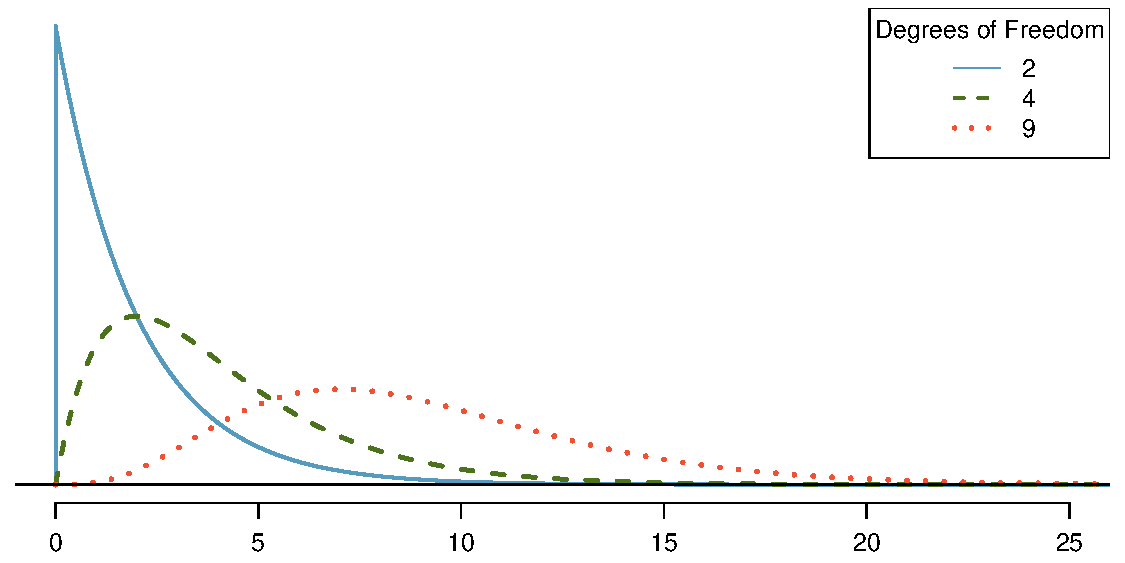
\includegraphics[width=0.9\textwidth]{05/figures/chiSquareDistributionWithInceasingDF/chiSquareDistributionWithInceasingDF}
\caption{Four chi-square distributions with varying degrees of freedom.}
\label{chiSquareDistributionWithInceasingDF}
\end{figure}

Figure~\ref{chiSquareDistributionWithInceasingDF} and Exercise~\ref{exerChiSquareDistributionDescriptionWithMoreDOF} demonstrate three general properties of chi-square distributions as the degrees of freedom increases: the distribution becomes more symmetric, the center moves to the right, and the variability inflates.

Our principal interest in the chi-square distribution is the calculation of p-values, which (as we have seen before) is related to finding the relevant area in the tail of a distribution. To do so, a new table is needed: the \term{chi-square probability table}, partially shown in Table~\ref{chiSquareProbabilityTableShort}. A more complete table is presented in Appendix~\ref{chiSquareProbabilityTable} on page~\pageref{chiSquareProbabilityTable}. This table differs a bit from the normal probability table, in that we typically do not find the tail area very precisely. Instead, we identify a range for the area. Additionally, the chi-square probability table only provides upper tail values as opposed to the normal probability table, which shows lower tail areas.

\begin{table}[h]
\centering
\begin{tabular}{r | rrrr | rrrr |}
  \hline
Upper tail & 0.3 & 0.2 & 0.1 & 0.05 & 0.02 & 0.01 & 0.005 & 0.001 \\ 
  \hline
df \hfill 1 & \footnotesize 1.07 & \footnotesize 1.64 & \footnotesize 2.71 & \footnotesize 3.84 & \footnotesize 5.41 & \footnotesize 6.63 & \footnotesize 7.88 & \footnotesize 10.83 \\ 
  2 & \footnotesize 2.41 & \footnotesize \color{tableHLBlue} 3.22 & \footnotesize \color{tableHLBlue} 4.61 & \footnotesize 5.99 & \footnotesize 7.82 & \footnotesize 9.21 & \footnotesize 10.60 & \footnotesize 13.82 \\ 
  \em3 & \em\footnotesize 3.66 & \em\footnotesize 4.64 & \em\footnotesize \textbf{\color{highlight}6.25} & \em\footnotesize 7.81 & \em\footnotesize 9.84 & \em\footnotesize 11.34 & \em\footnotesize 12.84 & \em\footnotesize 16.27 \\ 
  4 & \footnotesize 4.88 & \footnotesize 5.99 & \footnotesize 7.78 & \footnotesize 9.49 & \footnotesize 11.67 & \footnotesize 13.28 & \footnotesize 14.86 & \footnotesize 18.47 \\ 
  5 & \footnotesize 6.06 & \footnotesize 7.29 & \footnotesize 9.24 & \footnotesize 11.07 & \footnotesize 13.39 & \footnotesize 15.09 & \footnotesize 16.75 & \footnotesize 20.52 \\ 
  \hline
  6 & \footnotesize 7.23 & \footnotesize 8.56 & \footnotesize 10.64 & \footnotesize 12.59 & \footnotesize 15.03 & \footnotesize 16.81 & \footnotesize 18.55 & \footnotesize 22.46 \\ 
  7 & \footnotesize 8.38 & \footnotesize 9.80 & \footnotesize 12.02 & \footnotesize 14.07 & \footnotesize 16.62 & \footnotesize 18.48 & \footnotesize 20.28 & \footnotesize 24.32 \\ 
  \hline
\end{tabular}
\caption{A section of the chi-square probability table. A complete table is in Appendix~\ref{chiSquareProbabilityTable} on page~\pageref{chiSquareProbabilityTable}.}
\label{chiSquareProbabilityTableShort}
\end{table}

\begin{example}{Figure~\ref{chiSquareAreaAbove6Point25WithDF3} shows a chi-square distribution with 3 degrees of freedom and an upper shaded tail starting at 6.25. Use Table~\ref{chiSquareProbabilityTableShort} to estimate the shaded area.}
This distribution has three degrees of freedom, so only the row with 3 degrees of freedom (df) is relevant. This row has been italicized in the table. Next, we see that the value -- 6.25 -- falls in the column with upper tail area 0.1. That is, the shaded upper tail of Figure~\ref{chiSquareAreaAbove6Point25WithDF3} has area 0.1.
\end{example}

\begin{figure}
\centering
\subfigure[]{
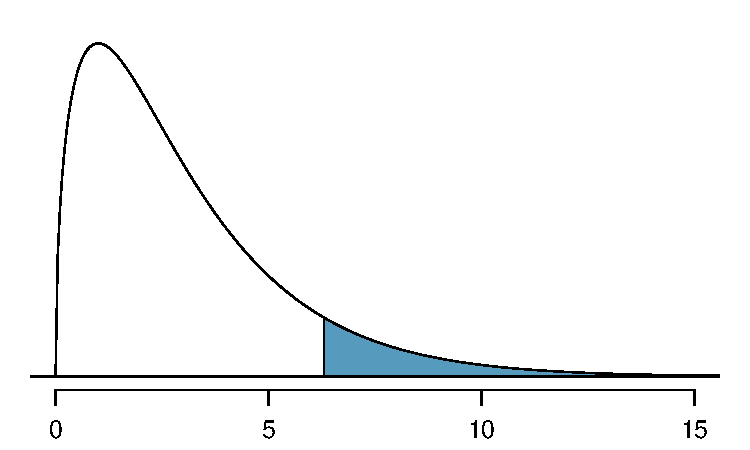
\includegraphics[width=0.475\textwidth]{05/figures/arrayOfFigureAreasForChiSquareDistribution/chiSquareAreaAbove6Point25WithDF3/chiSquareAreaAbove6Point25WithDF3}
\label{chiSquareAreaAbove6Point25WithDF3}
}
\subfigure[]{
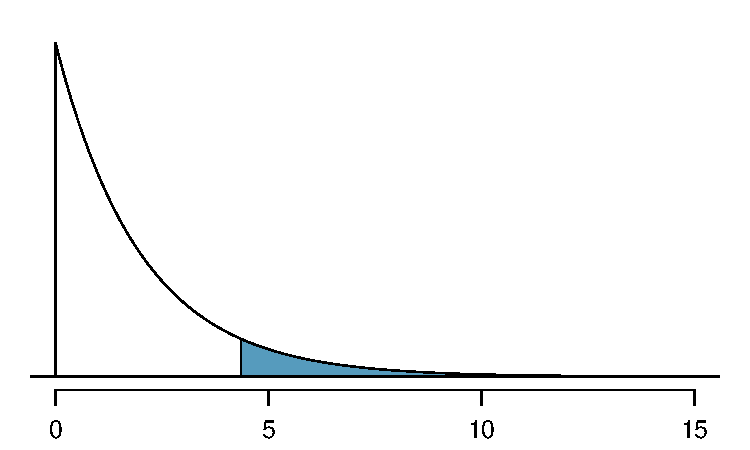
\includegraphics[width=0.475\textwidth]{05/figures/arrayOfFigureAreasForChiSquareDistribution/chiSquareAreaAbove4Point3WithDF2/chiSquareAreaAbove4Point3WithDF2}
\label{chiSquareAreaAbove4Point3WithDF2}
}
\subfigure[]{
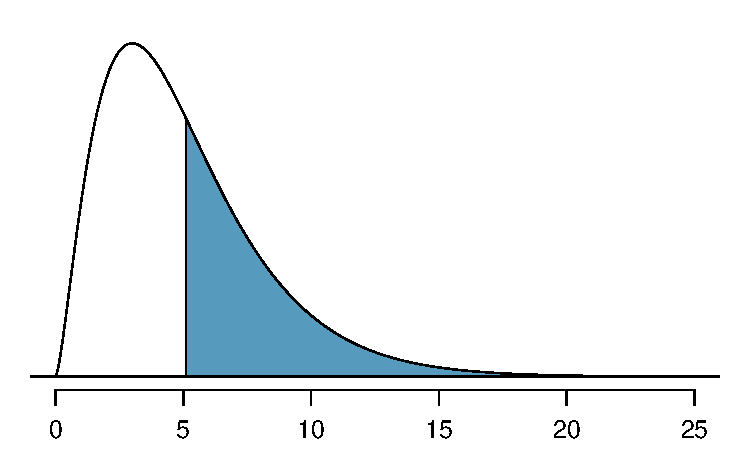
\includegraphics[width=0.475\textwidth]{05/figures/arrayOfFigureAreasForChiSquareDistribution/chiSquareAreaAbove5Point1WithDF5/chiSquareAreaAbove5Point1WithDF5}
\label{chiSquareAreaAbove5Point1WithDF5}
}
\subfigure[]{
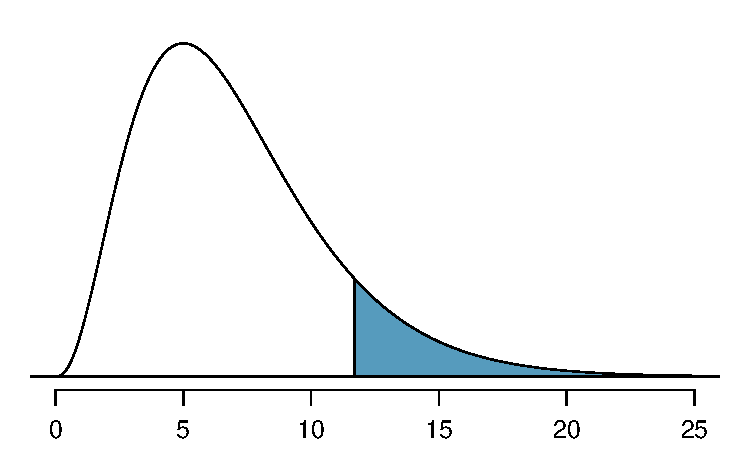
\includegraphics[width=0.475\textwidth]{05/figures/arrayOfFigureAreasForChiSquareDistribution/chiSquareAreaAbove11Point7WithDF7/chiSquareAreaAbove11Point7WithDF7}
\label{chiSquareAreaAbove11Point7WithDF7}
}
\subfigure[]{
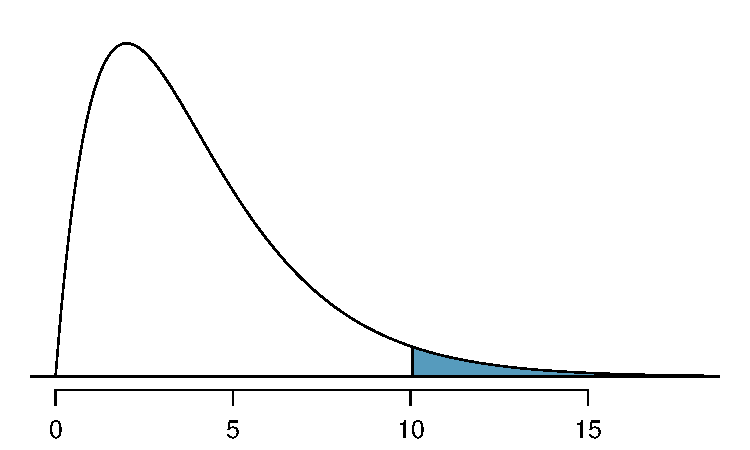
\includegraphics[width=0.475\textwidth]{05/figures/arrayOfFigureAreasForChiSquareDistribution/chiSquareAreaAbove10WithDF4/chiSquareAreaAbove10WithDF4}
\label{chiSquareAreaAbove10WithDF4}
}
\subfigure[]{
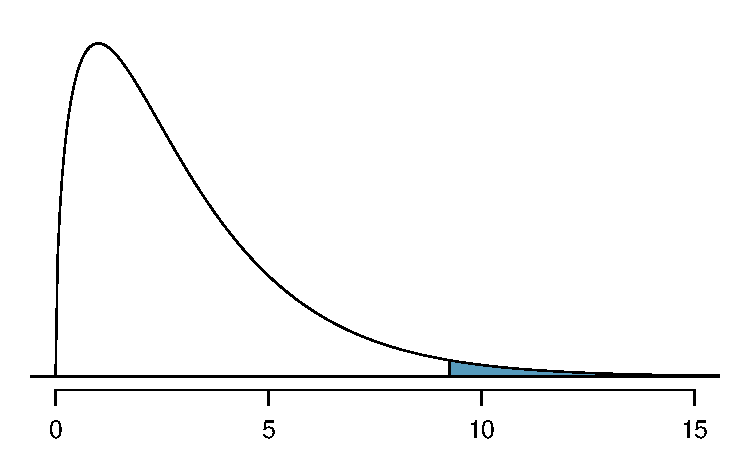
\includegraphics[width=0.475\textwidth]{05/figures/arrayOfFigureAreasForChiSquareDistribution/chiSquareAreaAbove9Point21WithDF3/chiSquareAreaAbove9Point21WithDF3}
\label{chiSquareAreaAbove9Point21WithDF3}
}
\caption{\textbf{\subref{chiSquareAreaAbove6Point25WithDF3}} Chi-square distribution with 3 degrees of freedom, area above 6.25 shaded. \textbf{\subref{chiSquareAreaAbove4Point3WithDF2}} 2 degrees of freedom, area above 4.3 shaded. \textbf{\subref{chiSquareAreaAbove5Point1WithDF5}} 5 degrees of freedom, area above 5.1 shaded. \textbf{\subref{chiSquareAreaAbove11Point7WithDF7}} 7 degrees of freedom, area above 11.7 shaded. \textbf{\subref{chiSquareAreaAbove10WithDF4}} 4 degrees of freedom, area above 10 shaded. \textbf{\subref{chiSquareAreaAbove9Point21WithDF3}} 3 degrees of freedom, area above 9.21 shaded.}
\label{arrayOfFigureAreasForChiSquareDistribution}
\end{figure}

\begin{example}{We rarely observe the \emph{exact} value in the table. For instance, Figure~\ref{chiSquareAreaAbove4Point3WithDF2} shows the upper tail of a chi-square distribution with 2 degrees of freedom. The bound for this upper tail is at 4.3, which does not fall in Table~\ref{chiSquareProbabilityTableShort}.}
The cutoff of interest -- 4.3 -- falls between the second and third columns in the 2 degrees of freedom row. Because these columns correspond to tail areas of 0.2 and 0.1, we can be certain that the area shaded in Figure~\ref{chiSquareAreaAbove4Point3WithDF2} is between 0.1 and 0.2.
\end{example}

\begin{example}{Figure~\ref{chiSquareAreaAbove5Point1WithDF5} shows an upper tail area for a chi-square distribution with 5 degrees of freedom and a cutoff of 5.1. Find the tail area.}
Looking in the row with 5 df, 5.1 falls below the smallest cutoff for this row (6.06). That means we can only say that the area is \emph{greater than 0.3}.
\end{example}

\begin{exercise}
Figure~\ref{chiSquareAreaAbove11Point7WithDF7} shows a cutoff of 11.7 on a chi-square distribution with 7 degrees of freedom. Find the area of the upper tail. Answer in the footnote\footnote{The value 11.7 falls between 9.80 and 12.02 in the 7 df row. Thus, the area is between 0.1 and 0.2.}.
\end{exercise}

\begin{exercise}
Figure~\ref{chiSquareAreaAbove10WithDF4} shows a cutoff of 10 on a chi-square distribution with 4 degrees of freedom. Find the area of the upper tail. Short answer in the footnote\footnote{The area is between 0.02 and 0.05.}.
\end{exercise}

\begin{exercise}
Figure~\ref{chiSquareAreaAbove9Point21WithDF3} shows a cutoff of 9.21 with a chi-square distribution with 3 df. Find the area of the upper tail. Short answer in the footnote\footnote{Between 0.02 and 0.05.}.
\end{exercise}



\subsection{Finding a p-value for a chi-square test}
\label{pValueForAChiSquareTest}

In Section~\ref{chiSquareTestStatistic}, we identified a new test statistic ($X^2$) within the context of assessing whether there was evidence of racial bias in how jurors were sampled. The null hypothesis represented the claim that jurors were randomly sampled and there was no racial bias. The alternative hypothesis was that there was racial bias in how the jurors were sampled.

We determined that a large $X^2$ value would suggest strong evidence favoring the alternative hypothesis: that there was racial bias. However, we could not quantify what the chance was of observing such a large test statistic ($X^2=5.89$) if the null hypothesis actually was true. This is where the chi-square distribution becomes useful. If the null hypothesis was true and there was no racial bias, then $X^2$ would follow a chi-square distribution, in this case with three degrees of freedom. In general, the statistic $X^2$ follows a chi-square distribution with $k-1$ degrees of freedom, where $k$ is the number of bins.

\begin{example}{How many categories were there in the juror example? How many degrees of freedom should be associated with the chi-square distribution used for $X^2$?}
In the jurors example, there were $k=4$ categories: white, black, Hispanic, and other. According to the rule above, the test statistic $X^2$ should then follow a chi-square distribution with $k-1 = 3$ degrees of freedom if $H_0$ is true.
\end{example}

Just like we checked sample size conditions to use the normal model in earlier sections, we must also check a sample size condition to safely apply the chi-square distribution for $X^2$. Each expected count must be at least\footnote{Some books recommend a threshold of 5.} 10. In the juror example, the expected counts were 198, 19.25, 33, and 24.75, all easily above 10, so we can apply the chi-square model to the test statistic, $X^2=5.89$.

\begin{example}{If the null hypothesis were true, the test statistic $X^2=5.89$ would be closely associated with a chi-square distribution with three degrees of freedom. Using this distribution and test statistic, identify the p-value.}
The chi-square distribution and p-value are shown in Figure~\ref{jurorHTPValueShown}. Because larger chi-square values correspond to stronger evidence against the null hypothesis -- i.e. larger deviations from what we expect -- we shade the upper tail to represent the p-value. Using the chi-square probability table in Appendix~\ref{chiSquareProbabilityTable} or the short table on page~\pageref{chiSquareProbabilityTableShort}, we can determine that the area is between 0.1 and 0.2. That is, the p-value is larger than 0.1 but smaller than 0.2. Generally we do not reject the null hypothesis with such a large p-value. In other words, the data do not provide convincing evidence of racial bias in the juror selection.
\end{example}

\begin{figure}
\centering
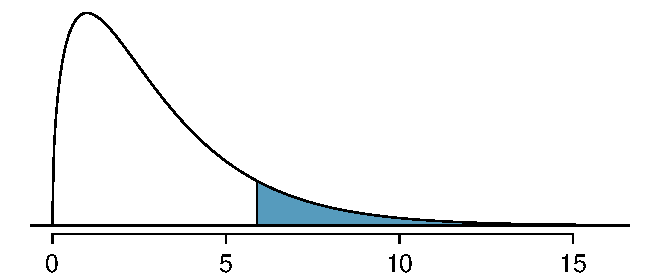
\includegraphics[width=0.57\textwidth]{05/figures/jurorHTPValueShown/jurorHTPValueShown}
\caption{The p-value for the juror hypothesis test is shaded in the chi-square distribution with $df=3$.}
\label{jurorHTPValueShown}
\end{figure}

\begin{termBox}{\tBoxTitle{Chi-square test for one-way table}
Suppose we are to evaluate whether there is convincing evidence that a set of observed counts $O_1$, $O_2$, ..., $O_k$ in $k$ categories are unusually different from what might be expected under a null hypothesis. Call the \emph{expected counts} that are based on the null hypothesis $E_1$, $E_2$, ..., $E_k$. If each expected count is at least 10 and the null hypothesis is true, then the following test statistic follows a chi-square distribution with $k-1$ degrees of freedom:
\begin{align*}
X^2 = \frac{(O_1 - E_1)^2}{E_1} + \frac{(O_2 - E_2)^2}{E_2} + \cdots + \frac{(O_k - E_k)^2}{E_k}
\end{align*}
The p-value for this test statistic is found by looking at the upper tail of this chi-square distribution. We consider the upper tail because larger values of $X^2$ would provide greater evidence against the null hypothesis.}
\end{termBox}

\begin{tipBox}{\tipBoxTitle{Conditions for the chi-square test}
There are two conditions that must be checked before performing a chi-square test:\vspace{-1mm}
\begin{description}
\setlength{\itemsep}{0mm}
\item[Independence.] Each case that contributes a count to the table must be independent of all the other cases in the table.
\item[Sample size / distribution.] Just like for proportions, each particular scenario (i.e. cell count) must have at least 10 cases. %If not, the distribution counts in the table may favor some cells so much that the test statistic doesn't closely follow the chi-square distribution under the null hypothesis.
\vspace{-1mm}
\end{description}
Failing to check conditions may unintentionally affect the test's error rates.}
\end{tipBox}

\vspace{-9mm}

\subsection{Evaluating goodness of fit for a distribution}

Section~\ref{geomDist} would be useful background reading for this example, but it is not a prerequisite.

We can apply our new chi-square testing framework to the second problem in this section: evaluating whether a certain statistical model fits a data set. Daily stock returns from the S\&P500 for 1990-2009 can be used to assess whether stock activity each day is independent of the stock's behavior on previous days. This sounds like a very complex question -- and it is -- but a chi-square test can be used to study the problem. We will label each day as \resp{Up} or \resp{Down} (\resp{D}) depending on whether the market was up or down that day. For example, consider the following changes in price, their new labels of up and down, and then the number of days that must be observed before each \resp{Up} day:
\begin{center}\footnotesize
\begin{tabular}{lc ccc ccc ccc cc}
Change in price		&\hspace{-1mm}	& \footnotesize2.52 &
	\footnotesize-1.46 & \footnotesize 0.51 &
	\footnotesize-4.07 & \footnotesize3.36 &
	\footnotesize1.10 &
	\footnotesize-5.46 & \footnotesize-1.03 & \footnotesize-2.99 & \footnotesize1.71 \\
Outcome	 & \hspace{-1mm} &
	\textbf{Up} &
	D & \textbf{Up} &
	D & \textbf{Up} &
	\textbf{Up} &
	D & D & D & \textbf{Up} \\
\footnotesize Days to \resp{Up} & \hspace{-1mm} & 1 & - & 2 & - & 2 & 1 & - & - & - & 4 \\
\end{tabular}
\end{center}
If the days really are independent, then the number of days until a positive trading day should follow a geometric distribution. The geometric distribution describes the probability of waiting for the $k^{th}$ trial to observe the first success. Here each \resp{Up} day represents a success, and down (\resp{D}) days represent failures. In the data above, it took only one day until the market was up, so the first wait time was 1 day. It took two more days before we observed our next \resp{Up} trading day, and two more for the third \resp{Up} day. We would like to determine if these counts (1, 2, 2, 1, 4, and so on) follow the geometric distribution. Table~\ref{sAndP500For1990To2009TimeToPosTrade} shows the number of waiting days for a positive trading day during 1990-2009 for the S\&P500.
\begin{table}[h]
\centering
\begin{tabular}{ll ccc ccc c ll}
\hline
Days	 & \hspace{2mm} & 1 & 2 & 3 & 4 & 5 & 6 & 7+ & \hspace{2mm} & Total \\
Observed &		& 1298 & 685 & 367 & 157 & 77 & 33 & 20 & & 2587 \\
\hline
\end{tabular}
\caption{Distribution of the waiting time until a positive trading day.}
\label{sAndP500For1990To2009TimeToPosTrade}
\end{table}

We consider how many days one must wait until observing an \resp{Up} day on the S\&P500 stock exchange. If the stock activity was independent from one day to the next and the probability of a positive trading day was constant, then we would expect this waiting time to follow a \emph{geometric distribution}. We can organize this into a hypothesis framework:
\begin{itemize}
\item[$H_0$:] Whether the stock market is up or down on a given day is independent from all other days. We will consider the number of days that pass until an \resp{Up} day is observed. Under this hypothesis, the number of days until an \resp{Up} day should follow a geometric distribution.
\item[$H_A$:] The days are not independent. Since we know the number of days until an \resp{Up} day would follow a geometric distribution under the null, we look for deviations from the geometric distribution, which would support the alternative hypothesis.
\end{itemize}
There are important implications in our result for stock traders: if information from past trading days is useful in telling what will happen today, that may provide an edge over other traders.

We consider data for the S\&P500 from 1990 to 2009 and summarize the waiting times in Table~\ref{sAndP500For1990To2009TimeToPosTrade2} and Figure~\ref{geomFitEvaluationForSP500For1990To2009}. The S\&P500 was positive on 52.9\% of those days.

\begin{table}
\centering
\begin{tabular}{ll ccc ccc c ll}
\hline
Days	 & \hspace{1mm} & 1 & 2 & 3 & 4 & 5 & 6 & 7+ & \hspace{1mm} & Total \\
\hline
Observed &		& 1298 & 685 & 367 & 157 & 77 & 33 & 20 & & 2587 \\
Geom. Model &		& 1368 & 644 & 304 & 143 & 67 & 32 & 28 & & 2587 \\
\hline
\end{tabular}
\caption{Distribution of the waiting time until a positive trading day. The expected counts based on the geometric model are shown in the last row. To find each expected count, we identify the probability of waiting $D$ days based on the geometric model ($P(D) = (1-0.529)^{D-1}(0.529)$) and multiply by the total number of streaks, 2587. For example, waiting for three days occurs under the geometric model about $0.471^2*0.529 = 11.7\%$ of the time, which corresponds to $0.117*2587 = 304$ streaks.}
\label{sAndP500For1990To2009TimeToPosTrade2}
\end{table}

\begin{figure}
\centering
\includegraphics[width=0.98\textwidth]{05/figures/geomFitEvaluationForSP500For1990To2009/geomFitEvaluationForSP500For1990To2009}
\caption{Side-by-side bar plot of the observed and expected counts for each waiting time.}
\label{geomFitEvaluationForSP500For1990To2009}
\end{figure}

Because applying the chi-square framework requires expected counts to be at least 10, we have \emph{binned} together all the cases where the waiting time was at least 7 days. The actual data, shown in the \emph{Observed} row in Table~\ref{sAndP500For1990To2009TimeToPosTrade2}, can be compared to the expected counts from the \emph{Geom. Model} row. The method for computing expected counts is discussed in Table~\ref{sAndP500For1990To2009TimeToPosTrade2}. In general, the expected counts are determined by (1) identifying the null proportion associated with each bin, then (2) multiplying each null proportion by the total count to obtain the expected counts. That is, this strategy identifies what proportion of the total count we would expect to be in each bin.

\begin{exercise}
Do you notice any unusually large deviations in the graph? Can you tell if these deviations are due to chance just by looking?
\end{exercise}

It is not obvious whether differences in the observed counts and the expected counts from the geometric distribution are significantly different. That is, it is not clear whether these deviations might be due to chance or whether they are so strong that the data provide convincing evidence against the null hypothesis. However, we can perform a chi-square test using the counts in Table~\ref{sAndP500For1990To2009TimeToPosTrade2}.

\begin{exercise}
Table~\ref{sAndP500For1990To2009TimeToPosTrade2} provides a set of count data for waiting times ($O_1=1298$, $O_2=685$, ...) and expected counts under the geometric distribution ($E_1=1368$, $E_2=644$, ...). Compute the chi-square test statistic, $X^2$. Answer in the footnote\footnote{$X^2=\frac{(1298-1368)^2}{1368} + \frac{(685-644)^2}{644} + \cdots + \frac{(20-28)^2}{28} = 24.43$}.
\end{exercise}

\begin{exercise}
Because the expected counts are all at least 10, we can safely apply the chi-square distribution to $X^2$. However, how many degrees of freedom should we use? Hint: How many groups are there? Solution in the footnote\footnote{There are $k=7$ groups, so we use $df=k-1=6$.}.
\end{exercise}

\begin{example}{If the observed counts follow the geometric model, then the chi-square test statistic $X^2=24.43$ would closely follow a chi-square distribution with $df=6$. Using this information, compute a p-value.} \label{RejectGeomModelForSP500StockDataFor1990To2009}
Figure~\ref{geomFitPValueForSP500For1990To2009} shows the chi-square distribution, cutoff, and the shaded p-value. If we look up the statistic $X^2=24.43$ in Appendix~\ref{chiSquareProbabilityTable}, we find that the p-value is less than 0.001. In other words, we have very strong evidence to reject the notion that the wait times follow a geometric distribution, i.e. trading days are not independent and past days may help predict what the stock market will do today.
\end{example}

\begin{figure}[h]
\centering
\includegraphics[width=0.8\textwidth]{05/figures/geomFitPValueForSP500For1990To2009/geomFitPValueForSP500For1990To2009}
\caption{Chi-square distribution with 6 degrees of freedom. The p-value for the stock analysis is shaded.}
\label{geomFitPValueForSP500For1990To2009}
\end{figure}

\begin{example}{In Example~\ref{RejectGeomModelForSP500StockDataFor1990To2009}, we rejected the null hypothesis that the trading days are independent. Why is this so important?}
Because the data provided strong evidence that the geometric distribution is not appropriate, we reject the claim that trading days are independent. While it is not obvious how to exploit this information, it suggests there are some hidden patterns in the data that could be interesting and possibly useful to a stock trader.
\end{example}

%%%%%%%%%
\section{Testing for independence in two-way tables (special topic)}
%\section{Two-way tables and chi-square (special topic)}
\label{twoWayTablesAndChiSquare}

Google is constantly running experiments to test new search algorithms. For example, Google might test three algorithms using a sample of 10,000 google.com search queries. Table~\ref{googleSearchAlgorithmByAlgorithmOnly} shows the 10,000 queries split into three algorithm groups\footnote{Google regularly runs experiments in this manner to help improve their search engine. It is entirely possible that if you perform a search and so does your friend, that you will have different search results. While the data presented in this section resemble what might be encountered in a real experiment, these data are simulated.}. The group sizes were specified before the start of the experiment to be 5000 for the current algorithm and 2500 for each test algorithm.

\begin{table}[h]
\centering
\begin{tabular}{ll ccc ll}
\hline
Search algorithm	 & \hspace{1mm} & current & test 1 & test 2 & \hspace{1mm} & Total \\
Counts &		& 5000 & 2500 & 2500 & & 10000 \\
\hline
\end{tabular}
\caption{Google experiment breakdown of test subjects into three search groups.}
\label{googleSearchAlgorithmByAlgorithmOnly}
\end{table}

%\begin{figure}[h]
%\centering
%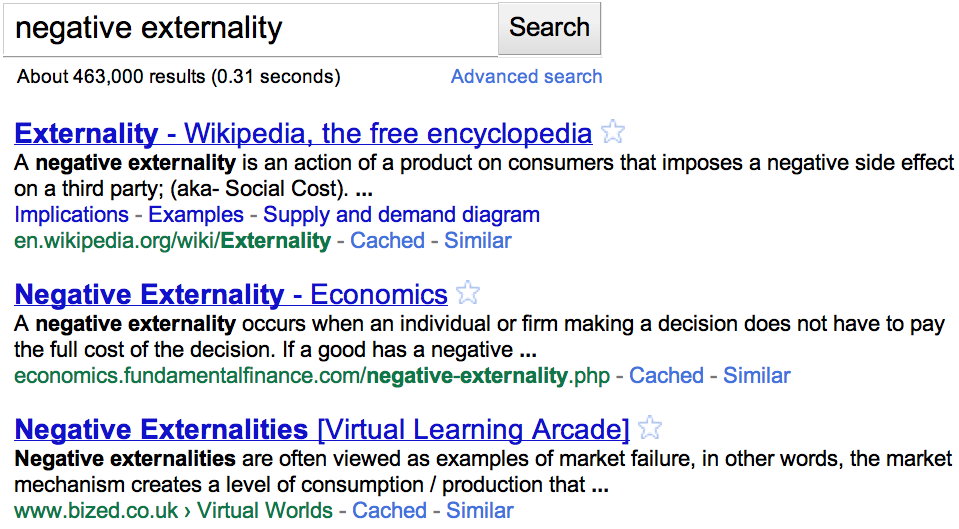
\includegraphics[width=0.85\textwidth]{05/figures/googleNegExtern}
%\caption{The first three search results on Google for \emph{negative externality}.}
%\label{googleNegExtern}
%\end{figure}

\begin{example}{What is the ultimate goal of the Google experiment? What are the null and alternative hypotheses, in regular words?}
The ultimate goal is to see whether there is a difference in the performance of the algorithms. The hypotheses can be described as the following:
\begin{itemize}
\item[$H_0$:] The algorithms each perform equally well.
\item[$H_A$:] The algorithms do not perform equally well.
\end{itemize}
\end{example}

In this experiment, the explanatory variable is the search algorithm. However, an outcome variable is also needed. This outcome variable should somehow reflect whether the search results align with the user's interests. One possible way to quantify this is to determine whether (1) the user clicked one of the links provided and did not try a new search, or (2) the user performed a related search. Under scenario (1), we might think that the user was satisfied with the search results. Under scenario (2), the search results probably were not relevant, so the user tried a second search.

Table~\ref{googleSearchAlgorithmByAlgorithmAndPerformanceWithTotals} provides the results from the experiment. These data are very similar to the count data in Section~\ref{oneWayChiSquare}. However, now the different combinations of two variables are binned in a \emph{two-way} table. In examining these data, we want to evaluate whether there is strong evidence that at least one algorithm is performing better than the others. To do so, we apply the chi-square test to this two-way table. The ideas of this test are similar to those ideas in the one-way table case. However, degrees of freedom and expected counts are computed a little differently than before.
\begin{table}[h]
\centering
\begin{tabular}{ll ccc ll}
\hline
Search algorithm & \hspace{1mm} & current & test 1 & test 2 & \hspace{1mm} & Total \\
\hline
No new search				   & & 3511    & 1749 & 1818 & 				& 7078 \\
New search				   & & 1489    & 751	& 682    &				& 2922 \\
\hline
Total						   & & 5000    & 2500 & 2500 & 				& 10000 \\
\hline
\end{tabular}
\caption{Results of the Google search algorithm experiment.}
\label{googleSearchAlgorithmByAlgorithmAndPerformanceWithTotals}
\end{table}

\begin{tipBox}{\tipBoxTitle[]{What is so different about one-way tables and two-way tables?}
A one-way table describes counts for each outcome in a single variable. A two-way table describes counts for \emph{combinations} of outcomes for two variables. When we consider a two-way table, we often would like to know, are these variables related in any way? That is, are they dependent (versus independent)?}
\end{tipBox}

The hypothesis test for this Google experiment is really about assessing whether there is statistically significant evidence that the choice of the algorithm affects whether a user performs a second search. In other words, the goal is to check whether the \var{search} variable is independent of the \var{algorithm} variable.

\subsection{Expected counts in two-way tables}

\begin{example}{From the experiment, we estimate the proportion of users who were satisfied with their initial search (no new search) as $7078/10000 = 0.7078$. If there really is no difference among the algorithms and 70.78\% of people are satisfied with the search results, how many of the 5000 folks in the current algorithm group would be expected to not perform a new search?} \label{googleExampleComputingTheExpectedNumberOfCurrentGroupWithNoNewSearch}
About 70.78\% of the 5000 would be satisfied with the initial search:
$$ 0.7078*5000 = 3539\text{ users} $$
That is, if there was no difference between the three groups, then we would expect 3539 of the current algorithm users not to perform a new search.
%then 3539 of the current algorithm users are not expected to perform a new search.
\end{example}

\begin{exercise}\label{googleExampleComputingTheExpectedNumberOfNewAlgGroupWithNoNewSearch}
Using the same rationale described in Example~\ref{googleExampleComputingTheExpectedNumberOfCurrentGroupWithNoNewSearch}, about how many users in each of the test groups would not perform a new search if the algorithms were equally helpful? Short answer in the footnote\footnote{About 1769.5. It is okay that this is a fraction.}.
\end{exercise}

\begin{example}{If 3539 of the 5000 users who are given the current algorithm are not expected to perform a new search, how many would we expect to perform a new search?} \label{googleExampleComputingTheExpectedNumberOfCurrentGroupWithNewSearch}
We would expect the other 1461 users in the ``current'' group to perform a new search.
\end{example}

\begin{exercise}\label{googleExampleComputingTheExpectedNumberOfNewAlgGroupWithNewSearch}
If 1769.5 of the 2500 users in each test group are not expected to perform a new search, how many would be expected to perform a new search in each of these groups? Answer in the footnote\footnote{$2500 - 1769.5 = 730.5$.}.
\end{exercise}

The expected counts from Examples~\ref{googleExampleComputingTheExpectedNumberOfCurrentGroupWithNoNewSearch} and~\ref{googleExampleComputingTheExpectedNumberOfCurrentGroupWithNewSearch} and Exercises~\ref{googleExampleComputingTheExpectedNumberOfNewAlgGroupWithNoNewSearch} and~\ref{googleExampleComputingTheExpectedNumberOfNewAlgGroupWithNewSearch} were used to construct Table~\ref{googleSearchAlgorithmByAlgorithmAndPerformanceWithExpectedCounts}. This is the same as Table~\ref{googleSearchAlgorithmByAlgorithmAndPerformanceWithTotals}, except now the expected counts have been added in parentheses.
\begin{table}[h]
\centering
\begin{tabular}{l lll lll lll l}
\hline
Search algorithm\hspace{2mm} & \multicolumn{2}{l}{current} &&
					\multicolumn{2}{l}{test 1} &&
					\multicolumn{2}{l}{test 2} & \hspace{0mm} & Total \\
\hline
No new search		   & 3511 &\color{steelBlue}\footnotesize(3539)    &&
					1749 &\color{steelBlue}\footnotesize(1769.5)	&&
					1818 &\color{steelBlue}\footnotesize(1769.5) &	& 7078 \\
New search		   & 1489 &\color{steelBlue}\footnotesize(1461)    && 
					751 &\color{steelBlue}\footnotesize(730.5)	&& 
					682 &\color{steelBlue}\footnotesize(730.5)    &		& 2922 \\
\hline
Total				   & 5000 &&& 	2500 &&& 	2500 &&& 	10000 \\
\hline
\end{tabular}
\caption{The observed counts and the {\color{steelBlue}(expected counts)}.}
\label{googleSearchAlgorithmByAlgorithmAndPerformanceWithExpectedCounts}
\end{table}

The examples and exercises above provided some help in computing expected counts. In general, expected counts for a two-way table may be computed using only the row totals, column totals, and the table total. For instance, if there was no difference between the groups, then about 70.78\% of each column should be in the first row:
\begin{align*}
0.7078*(\text{column 1 total}) &= 3539 \\
0.7078*(\text{column 2 total}) &= 1769.5 \\
0.7078*(\text{column 3 total}) &= 1769.5
\end{align*}
Looking back to how the fraction 0.7078 was computed -- as the fraction of users who did not perform a new search ($7078/10000$) -- these three expected counts could have been computed as
\begin{align*}
\left(\frac{\text{row 1 total}}{\text{table total}}\right)\text{(column 1 total)} &= 3539 \\
\left(\frac{\text{row 1 total}}{\text{table total}}\right)\text{(column 2 total)} &= 1769.5 \\
\left(\frac{\text{row 1 total}}{\text{table total}}\right)\text{(column 3 total)} &= 1769.5
\end{align*}
This leads us to a general formula for computing expected counts in a two-way table when we would like to test whether there is strong evidence of an association between the column variable and row variable.

\begin{termBox}{\tBoxTitle{Computing expected counts in a two-way table}
To identify the expected count for the $i^{th}$ row and $j^{th}$ column, compute
$$\text{Expected Count}_{\text{row }i,\text{ col }j} = \frac{(\text{row $i$ total}) * (\text{column $j$ total})}{\text{table total}}\vspace{2mm}$$}
\end{termBox}

\subsection{The chi-square test statistic for two-way tables}

The chi-square test statistic for a two-way table is found the same way it is found for a one-way table. For each table count, compute
\begin{align*}
&\text{General formula}& &\frac{(\text{observed count } - \text{ expected count})^2}{\text{expected count}} \\
&\text{Row 1, Col 1}& &\frac{(3511 - 3539)^2}{3539} = 0.222 \\
&\text{Row 1, Col 2}& &\frac{(1749 - 1769.5)^2}{1769.5} = 0.237 \\
& \vdots & &\hspace{13mm}\vdots \\
&\text{Row 2, Col 3}& &\frac{(682 - 730.5)^2}{730.5} = 3.220
\end{align*}
Adding the computed value for each cell gives the chi-square test statistic $X^2$:
$$X^2 = 0.222 + 0.237 + \dots + 3.220 = 6.120$$
Just like before, this test statistic follows a chi-square distribution. However, the degrees of freedom are computed a little differently for a two-way table\footnote{Recall: in the one-way table, the degrees of freedom was the number of cells minus 1.}. For two way tables, the degrees of freedom is equal to
\begin{align*}
df = \text{(number of rows minus 1)}*\text{(number of columns minus 1)}
\end{align*}
In our example, the degrees of freedom parameter is
\begin{align*}
df = (2-1)*(3-1) = 2
\end{align*}
If the null hypothesis is true (i.e. the algorithms are equally useful), then the test statistic $X^2 = 6.12$ closely follows a chi-square distribution with 2 degrees of freedom. Using this information, we can compute the p-value for the test, which is depicted in Figure~\ref{googleHTForDiffAlgPerformancePValue}.

\begin{termBox}{\tBoxTitle{Computing degrees of freedom for a two-way table}
When applying the chi-square test to a two-way table, we use
$$ df = (R-1)*(C-1) $$
where $R$ is the number of rows in the table and $C$ is the number of columns.}
\end{termBox}

\begin{figure}[h]
\centering
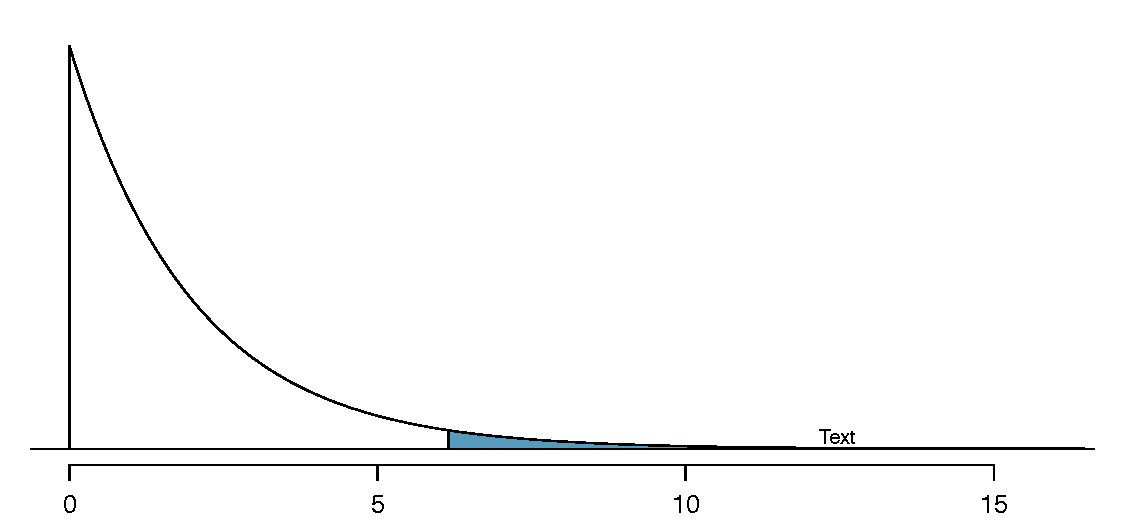
\includegraphics[width=0.7\textwidth]{05/figures/googleHTForDiffAlgPerformancePValue/googleHTForDiffAlgPerformancePValue}
\caption{Computing the p-value for the Google hypothesis test.}
\label{googleHTForDiffAlgPerformancePValue}
\end{figure}

\begin{example}{Compute the p-value and draw a conclusion about whether the search algorithms have different performances.}
Looking in Appendix~\ref{chiSquareProbabilityTable} on page~\pageref{chiSquareProbabilityTable}, we examine the row corresponding to 2 degrees of freedom. The test statistic, $X^2=6.120$, falls between the fourth and fifth columns, which means the p-value is between 0.02 and 0.05. Because we typically test at a significance level of $\alpha=0.05$ and the p-value is less than 0.05, the null hypothesis is rejected. That is, the data provide convincing evidence that there is some difference in performance among the algorithms.
\end{example}

\begin{example}{Table~\ref{pewResearchPollOnApprovalRatingsForChiSquareSectionExampleAndExercises} summarizes the results of a Pew Research poll\footnote{See the Pew Research website: {\scriptsize\urlwofont{http://people-press.org/report/598/healthcare-reform}}}. We would like to determine if there are actually differences in the approval ratings of Barack Obama, the Democratic leaders, and the Republican leaders. What are appropriate hypotheses for such a test?}\label{hypothesisTestSetupForPewResearchPollOnApprovalRatingsForChiSquareSection}
\begin{itemize}
\item[$H_0$:] There is no difference in approval ratings between the three groups.
\item[$H_A$:] There is some difference in approval ratings between the three groups, e.g. perhaps Obama's approval differs from other Democratic leaders.
\end{itemize}
\end{example}
\begin{table}
\centering
\begin{tabular}{ll ccc ll}
\hline
 & \hspace{1mm} & Obama & Dem. leaders & Rep. leaders & \hspace{1mm} & Total \\
\hline
Approve				   & & 683    & 465 & 375   & 				& 1523 \\
Disapprove			   & & 639    & 855 & 682   &				& 2379 \\
\hline
Total					   & & 1322    & 1320 & 1260 & 				& 3902 \\
\hline
\end{tabular}
\caption{Pew Research poll results of a March 2010 poll.}
\label{pewResearchPollOnApprovalRatingsForChiSquareSectionExampleAndExercises}
\end{table}

\begin{exercise}
A chi-square test for a two-way table may be used to test the hypotheses in Example~\ref{hypothesisTestSetupForPewResearchPollOnApprovalRatingsForChiSquareSection}. As a first step, compute the expected values for each of the six table cells. The computations for the expected counts in the cells of the first column are shown in the footnote\footnote{The expected count for row one / column one is found by multiplying the row one total (1523) and column one total (1322), then dividing by the table total (3902): $\frac{1523*1322}{3902} = 516.0$. Similarly for the first column and the second row: $\frac{2379*1322}{3902} = 806.0$.}.
\end{exercise}

\begin{exercise}
Compute the chi-square test statistic. Solution in the footnote\footnote{For each cell, compute $\frac{(\text{obs} - \text{exp})^2}{exp}$. For instance, the first row and first column: $\frac{(683-516)^2}{516} = 54.0$. Adding the results of each cell gives the chi-square test statistic: {\scriptsize$X^2 = 54.0 + \cdots + 17.8 = 142.2$}.}.
\end{exercise}

\begin{exercise}
Because there are 2 rows and 3 columns, the degrees of freedom for the test is $df=(2-1)*(3-1) = 2$. Use $X^2=142.2$, $df=2$, and the chi-square table (page~\pageref{chiSquareProbabilityTable}) to evaluate whether to reject the null hypothesis. Answer in the footnote\footnote{The test statistic is larger than the right-most column of the $df=2$ row of the chi-square probability table, meaning the p-value is less than 0.001. That is, we reject the null hypothesis because the p-value is less than 0.05, and we conclude that Americans' approval has differences among the party leaders and the president.}.
\end{exercise}


